\chapter{Evaluierung der Programmiersprache Elm}
\label{sec:Evaluierung der Programmiersprache Elm}
Die Programmiersprache Elm wird mit Hilfe einer empirischen Analyse in Form der Entwicklung eines praktischen Beispieles evaluiert. Dabei wird ein fertiges Template einer \ac{SPA}, welches in \ac{HTML}, \ac{CSS} und \ac{JS} programmiert wurde, in nativen Elm-Code überführt, insofern möglich. Ausschließlich die vorhandenen \ac{JS} und \ac{CSS}-Dateien sollen bestehen bleiben. Zur aussagekräftigen Evaluierung der Programmiersprache Elm hinsichtlich einer Nutzung im Bereich der Webentwicklung bedarf es zunächst einiger Bewertungskriterien, anhand derer eine Aussage möglich ist. Nachdem ein Bewertungsmuster erstellt und erläutert wurde, befasst sich der darauf folgende Teil der wissenschaftlichen Arbeit mit der Überführung des Templates in nativen Elm-Code. Zuletzt werden Beobachtungen, die während der Entwicklung auftraten, erläutert und die zuvor erörterten Kriterien ausgewertet. Das Kapitel mündet schließlich in einem Fazit, in dem sämtliche Beobachtungen, die Auswertung anhand der Bewertungskriterien abschließend wertend zusammengefasst werden.

\section{Bewertungsmuster}
\label{sec:Bewertungsmuster}
Das fertige Template ist eine \ac{SPA} mit Elementen, wie sie typischerweise auf einer solchen Webseite vertreten sind. Eine \ac{SPA} ist, wie der Name bereits suggeriert, eine Webseite mit effektiv nur einer aktiven Seite und ohne Unterseiten (ausgenommen Impressum, AGB und Datenschutz). Die \ac{SPA} wird genutzt um ein Produkt oder Konzept schnell und einfach zu präsentieren, ohne den Nutzer mit Informationen zu überfluten und Unübersichtlichkeit in Form von tief verlinkten Unterseiten zu erzeugen. Oftmals wird eine SPA auch als Startseite benutzt und bietet nur eine geringe Anzahl an Funktionen.
Die fertige \ac{SPA} soll unter anderem die folgenden, typischen Elemente enthalten:
\begin{itemize}
	\item Navigation mit Anchor-Elementen
	\subitem{-} Verkleinern der Navigation nach $x$ Pixeln
	\subitem{-} ScrollSpy zur Darstellung der aktuellen Position
	\item Titelbild mit einem vertikal und horizontal zentriertem Text
	\item Service-Sektion
	\item Twitter-Bootstrap-\ac{CSS} mitsamt allen Funktionen
	\subitem{-} Vorgefertiges, responsive Design
	\subitem{-} Aufklappbares Menü
	\item Portfolio mit Bildern, wobei ein Klick einen asynchronen Request ausführt und Daten nach lädt
	\item Formular zur Kontaktaufnahme mit Validierung der eingegebenen Daten
\end{itemize}
Mit diesen Elementen kann eine typische SPA verwirklicht werden. Die Navigation bietet dabei die Möglichkeit für den Nutzer schnell zwischen einzelnen Sektionen der Seite zu wechseln. Das initiale Titelbild mit einem zentrierten Text gibt den Kontext der Präsentation an und soll das Interesse des Nutzers anregen. Die folgende Service-Sektion wird dazu genutzt, allgemeine Informationen über das beworbene Produkt anzuzeigen. In der darauf folgenden Portfolio-Sektion werden dem Nutzer mehrere Bilder des Produktes angezeigt, wobei ein Klick auf eines der Bilder dazu führt, dass ein Popup erzeugt wird, in welches mit Hilfe eines AJAX-Requests Informationen asynchron vom Server angefordert und im Nachhinein geladen werden. Zuletzt kann sich der Nutzer ein Kontaktformular ausfüllen, das auf Korrektheit hin überprüft wird.


\section{Bewertungskriterien}
\label{sec:Bewertungskriterien}
Während der Überführung des Templates soll der erzeugte Code, sowie der Weg dahin analysiert werden. Hierbei sind Aspekte wie Wiederverwendbarkeit und Effizienz von großer Bedeutung. Aber auch die Produktivität während der Arbeit mit dem Code soll betrachtet werden. Die Bewertungskriterien setzen sich zum Großteil aus den zugrunde liegenden Kriterien aus dem Dokument XY der Washington University zusammen. Im Folgenden soll die Notwendigkeit der Kriterien und ihre eigentliche Bedeutung verständlich gemacht werden.

%TODO: http://www.cs.gordon.edu/courses/cs323/lectures-2009/LanguageEvaluationCriteria.pdf\\
%http://courses.cs.washington.edu/courses/cse341/02sp/concepts/evaluating-languages.html

%\subsection{Entwicklungsgeschwindigkeit}
%\label{sec:Entwicklungsgeschwindigkeit}
%Gerade für Startups ist es wichtig, ein erstes Produkt so schnell wie möglich bereitzustellen. Die Entwickler müssen entsprechend mit wenigen Mitteln ein fertiges (Software-)Produkt ausliefern können, selbst wenn sie noch kein oder wenig Vorwissen zu einer Programmiersprache haben.
%Dementsprechend sollte eine Programmiersprache nur eine geringe Anzahl an primitiven Konzepten aufweisen, die sich leicht erweitern lassen. Beispielsweise hat die Programmiersprache $C$ standardmäßig keine Anreihung von Buchstaben, auch bekannt als $String$. Jedoch gibt es den Datentyp $char$, der einen einzelnen Buchstaben repräsentiert. Durch die Verknüpfung mehrerer $char$'s, kann letztendlich der Datentyp $String$ umgesetzt werden. 
%TODO: Weg, oder re-write. Bibliotheken erlauben üblicherweise schnelleres/leichteres programmieren, aufgrund der Sammlung von Algorithmen.


\subsection{Wartbarkeit und Lesbarkeit}
\label{sec:Wartbarkeit}
Es ist unabdingbar, dass verfasster Quellcode wartbar ist. Dazu gehört einerseits, dass der Code lesbar ist, unabhängig von der Zeit die sich ein Entwickler bereits mit der Codebasis auseinandergesetzt hat. Damit Quellcode lesbarer wird, reicht es schon aus Kommentare im Code zuzulassen, die beispielsweise eine Funktion und ihr Ziel beschreiben, oder wichtige Informationen über einen Algorithmus enthalten. Des Weiteren sollten Funktionen und Variablen kurze und prägnante Namen haben, wodurch die Verständlichkeit des Quellcodes unterstützt wird. Die Programmiersprache Elm kann als wartbar bezeichnet werden, insofern es Möglichkeiten zum Kommentieren des Codes gibt, oder bestenfalls automatisch Informationen in Form von Kommentaren über Funktionen und Verhaltensweisen von Algorithmen generiert werden.


\subsection{Zuverlässigkeit}
\label{sec:Zuverlässigkeit}
Für einen Entwickler von Software ist es wichtig, dass das ausgelieferte Programm letzten Endes fehlerfrei funktioniert. Dazu gehört, dass das Programm nicht unvorhergesehen abstürzt, andere Systeme beeinträchtigt, oder dem späteren Nutzer der Software anderweitig Probleme beschert. In den meisten Fällen helfen die Editoren mit denen der Quellcode geschrieben wird bereits, indem syntaktische Fehler durch Markierungen sichtbar, oder Vorschläge zur Vervollständigung des angefangenen Codes gemacht werden. Wichtig ist entsprechend, dass die Programmiersprache auf offensichtliche Fehler, entweder durch Plugins für den Editor oder durch den Compiler selbst, aufmerksam macht und sie somit verhindert und nicht erst im Produktionssystem den Fehler zulässt. Als Testfall wird Quellcode bewusst mit Fehlern versehen, die zu einem Absturz des Programmes während der Laufzeit führen würden. Erkennt der $elm-compiler$ diese Fehler oder umgeht den Absturz, gilt das Kriterium als erfüllt.


\subsection{Portabilität}
\label{sec:Portabilität}
Nicht alle Programmiersprachen und die damit erzeugten Programme funktionieren auf allen Endgeräten. Es kommt dabei sehr stark auf die Hardwarekomponenten und das Betriebssystem des Zielsystems an. Es ist wünschenswert, dass Quellcode nur einmal geschrieben und auf das Zielsystem übertragen werden kann, ohne großartige Änderungen am Quellcode vornehmen zu müssen. Letzten Endes wird versucht den Quellcode auf mehreren Zielsystemen zu kompilieren. Elm liefert Installationsanweisungen für die Betriebssysteme $Mac$, $Windows$ und allen Betriebssystemen, die $nodejs$ unterstützen. Gibt es keinerlei Differenz in Form von Fehlern oder Warnungen während des Kompilierens, gilt die Portabilität als erfüllt.


\subsection{Effizienz}
\label{sec:Effizienz}
„Zeit ist Geld.“ ist auch heute noch immer eine wahre Aussage. Entsprechend ist es von Vorteil, wenn Quellcode schnell erzeugt, getestet und als fertiges Produkt (Software) an den Kunden ausgeliefert werden kann. Dabei ist es wichtig, dass der Compiler den Quellcode schnell in ein lauffähiges Programm verwandelt und auch das daraus resultierende Programm effizient arbeitet, sprich schnell ist. Damit eine Aussage über die notwendige Zeit für das kompilieren des Quellcodes getroffen werden kann, wird der Code zehn mal kompiliert und die benötigte Zeit gemessen. Anschließend wird der höchste und niedrigste Wert verworfen. Um ein Caching durch den Compiler zu verhindern, wird vor jedem Kompiliervorgang die zuvor erzeugten Programmdateien gelöscht. Im Anschluss wird das arithmetische Mittel der verbleibenden acht Werte ermittelt. TODO.
Die Performance der Programmiersprache wird nicht anhand des hier entwickelten Projektes, sondern der externen Applikation \cite{https://github.com/evancz/todomvc-perf-comparison/} TodoMVC Performance Comparison ermittelt. Dieses Tool ermöglicht es, anhand der Beispiel-Applikation "TodoMVC", die in mehreren Programmiersprachen realisiert wurde, die Performance des Programmes in den einzelnen Programmiersprachen zu testen. Dabei werden automatisch gewisse Aktionen in der jeweiligen Sprache durchgeführt, die benötigte Zeit gemessen und die Ergebnisse am Ende gegenübergestellt. Mit Hilfe des Tools werden 20 Messungen durchgeführt und das Endergebnis betrachtet. Ist Elm signifikant schneller als der Großteil der anderen getesteten Programmiersprachen, gilt das Kriterium als erfüllt. Die anderen Umgebungen der Applikation sind ebenso in nativem \ac{JS} oder einer zu \ac{JS} kompilierenden Programmiersprache geschrieben. Dadurch kann eine Aussage über die tatsächliche Effizienz der Applikation im Vergleich gemacht werden.


\subsection{Wiederverwendbarkeit}
\label{sec:Wiederverwendbarkeit}
Vorhandene Codeteile neu zu verfassen oder händisch kopieren zu müssen ist sehr ineffizient. Besser ist es, wenn Funktionen mehrfach genutzt werden können. Auf diese Weise müssen Änderungen nicht mehrmals vorgenommen werden und die Fehleranfälligkeit sinkt. Ferner sollten Funktionen nicht nur wiederverwendbar, sondern isoliert in einem eigenen Modul definiert werden können. Besteht die Möglichkeit Module zu erstellen und diese an unterschiedlichen Stellen beliebig anzuwenden, gilt das Kriterium als erfüllt. Erweitert wird das Kriterium durch einen zusätzlichen Zugriffsschutz von außen, das bedeutet, dass innerhalb eines Moduls definiert werden kann, welche Funktionen nach außen hin sichtbar sind.


\section{Web-spezifische Bewertungskriterien}
\label{sec:web-kriterien}
Die bisherigen Kriterien ermöglichen es, die Programmiersprache als solches anhand der eingebauten Möglichkeiten die diese bietet objektiv beurteilen zu können. Da sich diese wissenschaftliche Arbeit allerdings ausdrücklich mit der Evaluierung von Elm für Webapplikationen auseinandersetzt, müssen auch diese Kriterien untersucht werden und einen höheren Stellenwert bei der Bewertung einnehmen.
Webapplikationen können grundsätzlich in zwei Typen unterteilt werden. Zunächst gibt es die \ac{SPA}, bestehend aus nur einer einzigen Seite, bei der typischerweise nur wenig  Programmlogik vorhanden ist und der Client lediglich die Informationen anzeigt. Des Weiteren gibt es die Rich-Internet-Applikationen\\
(RIA: http://www.itwissen.info/definition/lexikon/rich-Internet-application-RIA.html). Diese Art der Webapplikation besitzt im wesentlichen mehr Programmlogik, die der Client ausführen kann. Ein weiteres Merkmal sind oftmals auch die Anzahl der vorhandenen Unterseiten, wodurch wiederum mehr Logik erforderlich wird.
Bei der Erstellung einer \ac{SPA} muss generell weniger Aufwand betrieben werden, um eine fertige Präsentation zu erstellen.
Jede Webapplikation lebt von einem Frontend, sowie einem Backend. Typischerweise bezeichnet das Frontend dabei alle Komponenten, die an den Benutzeroberfläche des Nutzers gesendet werden. Dazu gehören unter anderem die Komponenten \ac{HTML}, \ac{CSS} und \ac{JS}. Der Nutzer interagiert mit dieser Darstellung der Oberfläche.
Das Gegenstück zum Frontend stellt das sogenannte Backend dar. Dabei handelt es sich um Komponenten, die dem Webserver zugehörig sind. Unter anderem ist das zum Beispiel eine Datenbank, die eigentliche Webapplikation und natürlich der Webserver selbst. Der Nutzer agiert mit dem Backend nur über zuvor im Frontend eingerichtete Schnittstellen.


\subsection{Browser Kompatibilität}
\label{sec:Browser Kompatibilität}
Ein weiterer wichtiger Aspekt ist die Kompatibilität der Browser mit den genutzten Programmiersprachen. Da der Browser die Darstellung des \ac{HTML} und \ac{CSS} Quellcodes übernimmt, sowie die Manipulationen des DOM durch \ac{JS}, ist es wichtig, dass der Browser den vorhandenen Quellcode lesen und ausführen kann. Sämtliche Sprachen wie \ac{HTML}, \ac{CSS} und \ac{JS} befinden sich im konstanten Wandel und werden stets weiter entwickelt.
Dabei werden nicht nur vorhandene Fehler behoben, sondern auch neue Eigenschaften hinzugefügt, sowie teilweise ersetzt oder verworfen. Diese Änderungen können darin münden, dass Nutzer unterschiedlicher Browser, auch unterschiedliche Ergebnisse angezeigt bekommen, manche Features gar nicht erst funktionieren oder die Applikation im schlimmsten Fall abstürzt. Dementsprechend ist es wichtig, dass die Applikation auf den gängigen Browsern fehlerfrei funktioniert, insbesondere den fünf meistgenutzten Browsern Google Chrome, Safari, Internet Explorer, Firefox und Opera (vgl. Abbildung~\ref{fig:browser-may-2016}). Sollte die Applikation fehlerfrei in allen Browsern starten und die Funktionalität vollends gegeben sein, kann dieses Kriterium als erfüllt angesehen werden.
\iffalse
www.w3counter.com/trends\\+
https://www.w3counter.com/globalstats.php?year=2016&month=5
\fi

\begin{figure}[hb]
  \centering  
  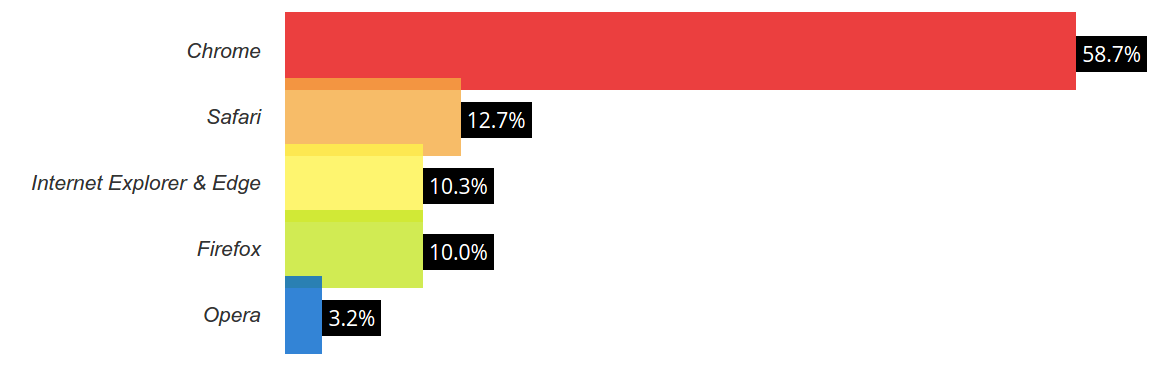
\includegraphics[scale=0.3]{img/browser_2016.png}
  \caption{Die fünf meistgenutzten Browser im Mai 2016 \cite{top-five-browser-statistics}}\label{fig:browser-may-2016}
\end{figure}

\subsection{Interoperabilität}
\label{sec:Interoperabilität_Analyse}
Auch bei den Webapplikationen ist es wichtig, bereits existente Frameworks und Problemlösungen nutzen zu können. Folglich müssen externe \ac{JS} und \ac{CSS} Bibliotheken ohne große Probleme eingebettet werden können, ohne den Quellcode zu verändern. Sollte es die Möglichkeit geben bestehende, externe Bibliotheken einzubinden oder anderweitig nutzbar zu machen, gilt das Kriterium als erfüllt.


\subsection{Asynchrone Verarbeitung}
\label{sec:Asynchrone Verarbeitung}
Große Datenmengen, deren Übertragung einige Sekunden in Anspruch nimmt, oder Aufgaben die langwierig sind, sollten nicht synchron ausgeführt werden. Stattdessen bietet es sich an, asynchrone Aufgabenblöcke zu definieren, wie beispielsweise das nachladen von Daten, sollten sie tatsächlich angefordert werden. Am Beispiel der hier geplanten \ac{SPA} bedeutet dies, dass Informationen von einem Webserver erst angefordert und sichtbar gemacht werden, sobald der Nutzer diese durch einen Klick auf ein Element anfordert. Da initial gewisse Daten noch nicht vorhanden sind, verringert sich die Datenmenge der zu übertragenen Informationen. Dadurch kann der Webserver entlastet und die initiale Ladezeit der Webseite verringert werden. Um das Kriterium der asynchronen Verarbeitung zu erfüllen, sollte Elm die Möglichkeit liefern, asynchrone Requests an einen Server zu schicken, Daten anzufordern und die Antwort darzustellen. Die Applikation darf dabei nicht in einen undefinierten Zustand kommen, sprich durch beispielsweise eine langsame Übertragungsrate Fehler bei der Darstellung erzeugen oder die Ausführung von nachfolgenden Operationen verzögern.


\subsection{Dateigröße}
\label{sec:Dateigroesse}
Die Größe einer Datei wirkt sich auf die Dauer der Übertragungszeit aus. Ist die Datenmenge groß, steigt entsprechend auch die Dateigröße an. Eine schlechte Übertragungsrate kann somit zu erheblichen Verzögerungen der fertigen Darstellung führen. Um die Dateigröße von üblichen \ac{JS}-Dateien zu verringern, werden oftmals externe Tools zur Entfernung von Leerzeichen oder der Verkürzung von Funktions- und Variablennamen genutzt. Für die anschließende Bewertung dieses Kriteriums, sollte der Compiler die Möglichkeit zur automatischen Verkleinerung der Dateigröße mit einer Effizienz von mindestens 50\% bieten. Zusätzlich sollte die Dateigröße eines Elm-Programmes mit den eingebundenen Standard-Bibliotheken $elm-lang/core$ und $elm-lang/html$ 150 Kilobyte nicht übersteigen.

\newpage
\section{Empirische Analyse}
\label{sec:Empirische Analyse}
Die folgende Sektion unterstützt und erläutert die praktische Ausarbeitung der \ac{SPA}. Dabei wird zunächst der typische Programmablauf der Applikation erörtert. Ferner wird die Entwicklungsumgebung unter der die Applikation ausgearbeitet wurde vorgestellt. Die Entwicklung wird in einzelne Abschnitte unterteilt und einzeln erläutert.

\subsection{Programmablauf}
\label{sec:Programmablauf}
Abbildung XY: Zeigt die Kommunikation zwischen Client und Webserver
Die Abbildung XY zeigt die geplante Kommunikation zwischen dem Client und dem Webserver.
In Schritt 1 fordert der Nutzer die Webseite an und erzeugt dadurch einen Request. Dieser geht in Schritt 2 bei dem Webserver ein und wird verarbeitet. Abhängig von der angeforderten URL erzeugt der Webserver eine Antwort, mit allen zu sendenden Informationen und dem dazugehörigen \ac{HTML}, \ac{CSS} und \ac{JS} Code. Im nächsten Schritt 3 werden diese Daten zurück an den Client gesendet. Der Client nimmt die Daten entgegen, wie in Schritt 4 beschrieben. Des Weiteren macht der Client die Daten entsprechend sichtbar, so dass der Nutzer eine vollständige Präsentation der Webseite sieht. Schritt 5 beschreibt die mögliche Interaktion des Nutzers mit dem ihm präsentierten Dokument. Jede Interaktion wird durch \ac{JS} erkannt und erzeugt eine Reaktion. Unter Umständen ist dies ein Request an den Server, womit bei Schritt 1 begonnen wird.


\subsection{Entwicklungsumgebung}
\label{sec:Entwicklungsumgebung}
Die zugrunde liegende Elm-Version ist 0.17 und wird unter Ubuntu 14.04 64bit installiert. Als Editor wird Atom mit den Elm-spezifischen Plugins $language-elm$, $linter-elm-make$ und $elm-format$ verwendet. Diese Plugins unterstützen die Entwicklung von Elm-Programmen, indem der Quellcode beim speichern automatisch dem Style-Guide entsprechend formatiert, eventuelle Fehler bei der Kompilierung direkt im Editor sichtbar gemacht und der Code syntaktisch gefärbt, sowie Vorschläge zur Vervollständigung des geschriebenen Quellcodes gemacht werden. Da die Pakete ständig aktualisiert und verändert werden, wird an dieser Stelle von einer detaillierten Beschreibung zur Installation und Verwendung abgesehen und auf die Dokumentationen der einzelnen Pakete verwiesen.
Der angefertigte Quellcode wird durch den Compiler $elm-make$ kompiliert.
Anschließend wird die fertige \ac{SPA} mit den Browsern Google Chrome (Version 51), Internet Explorer (Version XY), Mozilla Firefox (Version 47) und Opera (Version 38). In Bezug auf die Abbildung~\ref{fig:browser-may-2016} fällt auf, dass Safari als einziger der fünf meistgenutzten Browser nicht getestet wird. Zum Zeitpunkt dieser wissenschaftlichen Arbeit stand kein entsprechendes Testgerät zur Verfügung. Die in der Abbildung genannten Browser decken 94,9\% aller genutzten Browser ab. Abzüglich des Browsers Safari, werden entsprechend die verbleibenden 82,2\% aller Browser überprüft.


TODO: (https://github.com/triforkse/atom-elm-format)\\
(https://github.com/triforkse/atom-elm-format)\\
(https://atom.io/packages/language-elm\\

\subsection{Grundaufbau}
\label{sec:Grundaufbau}
Damit der Nutzer letzten Endes eine Webseite besuchen kann, muss zunächst ein auslieferbares Dokument erzeugt werden. Hierfür wird zunächst die $index.html$-Datei aus dem Template $Agency$ übernommen und entsprechend angepasst. Die Datei dient dabei als Grundgerüst für die Elm-Applikation und lädt externe \ac{CSS} und \ac{JS}-Dateien.
Zunächst wird sämtlicher Code Code der für die Darstellung des Templates innerhalb des $body$-Elementes definiert wurde entfernt. Lediglich die $script$-Tags bleiben innerhalb des $body$s bestehen, so dass sämtliche vordefinierte \ac{JS}-Dateien weiterhin geladen werden.
\begin{figure}[p]
\centering
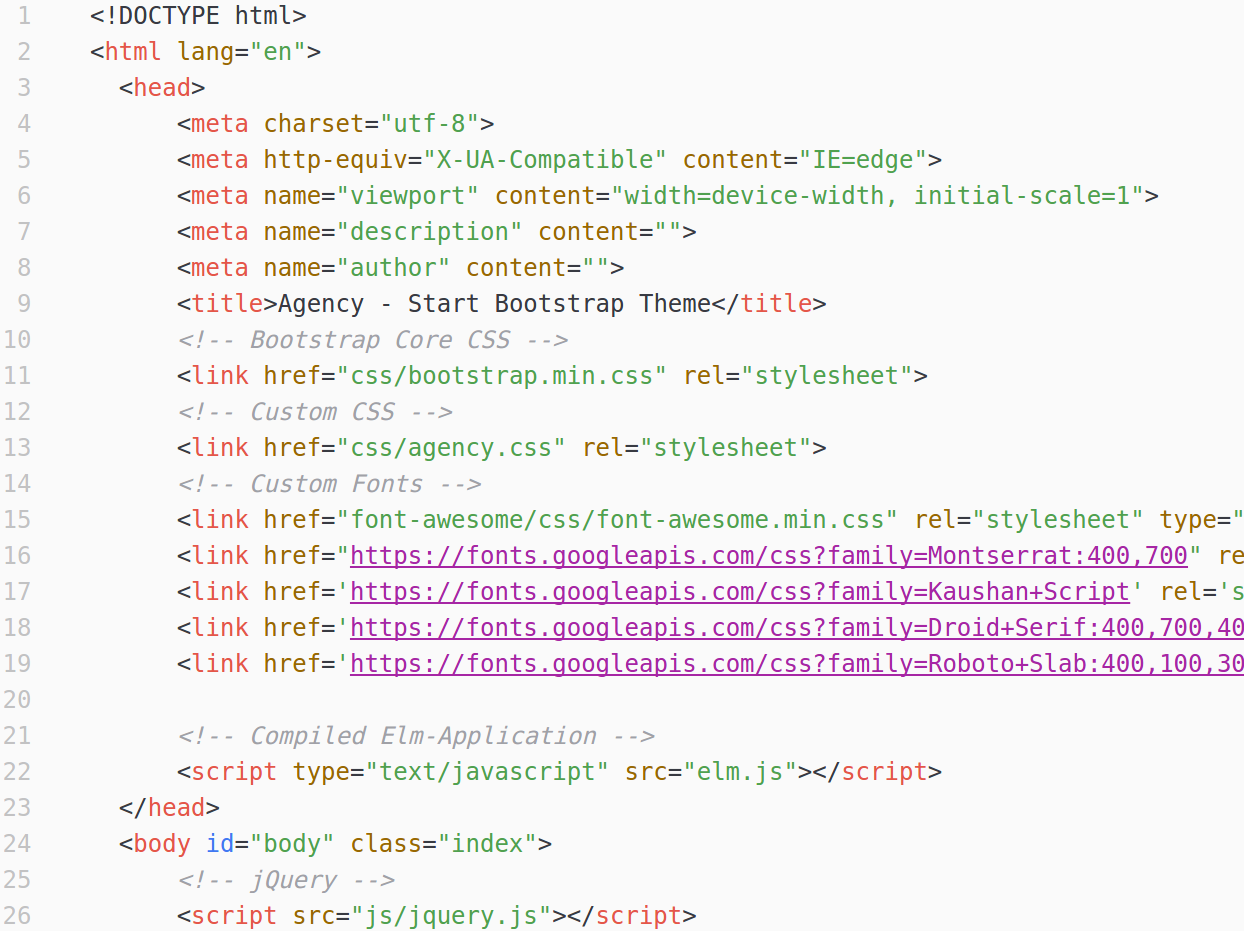
\includegraphics[scale=0.32]{img/index-grundaufbau-1.png}
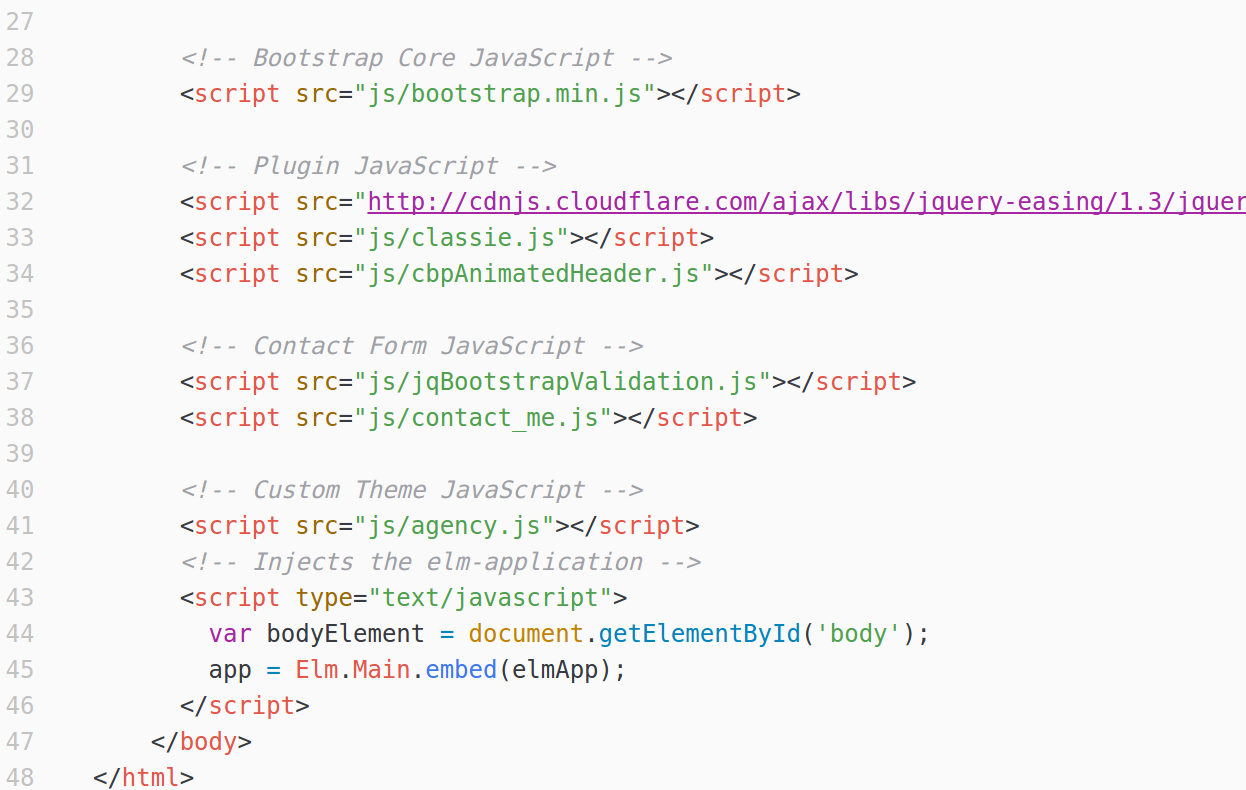
\includegraphics[scale=0.32]{img/index-grundaufbau-2.png}
\caption{Grundaufbau der $index.html$, um die Elm-Applikation zu injizieren}\label{fig:index-grundaufbau}
\end{figure}

\begin{figure}[p]
\centering
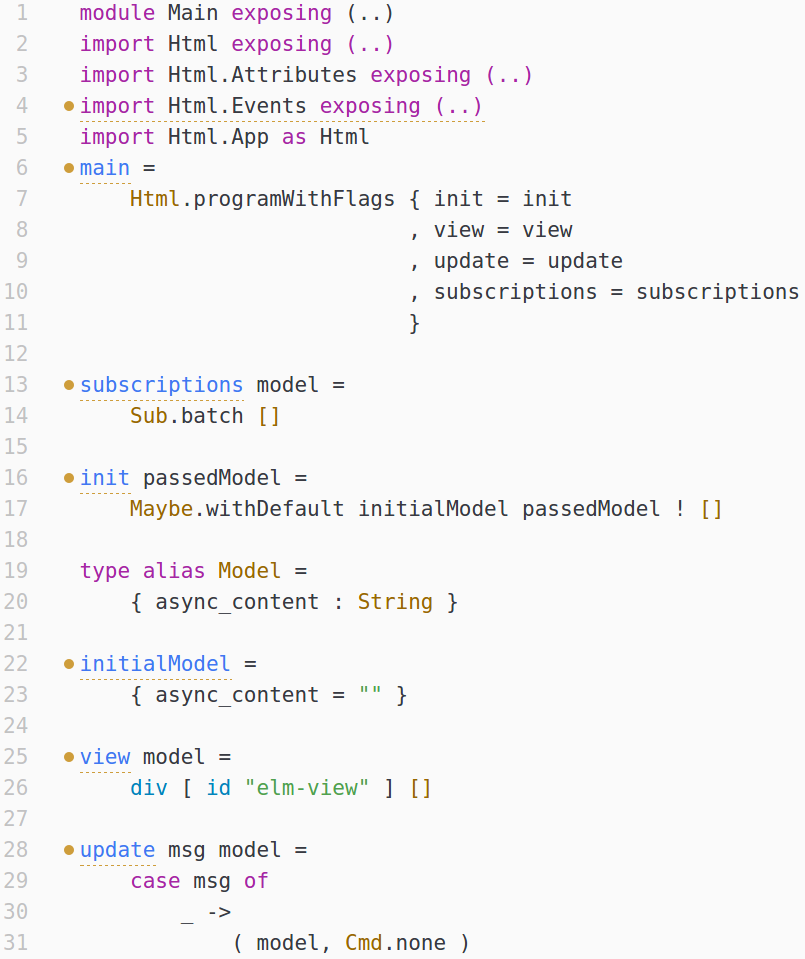
\includegraphics[scale=0.5]{img/elm-grundaufbau-start.png}
\caption{Grundgerüst der Elm-Applikation}\label{fig:elm-grundaufbau-start}
\end{figure}
Damit in das Grundgerüst die Elm-Applikation geladen werden kann, ist ein weiterer $script$-Tag notwendig, der die kompilierte Elm-Applikationsdatei $elm.js$ einbindet. Des Weiteren muss die Elm-Applikation explizit aufgerufen und gestartet werden. Die Abbildung~\ref{fig:index-grundaufbau} zeigt die $index.html$ mit den notwendigen Änderungen in Zeile $22$, in welcher die kompilierte Elm-Applikation eingebunden wird, sowie den Zeilen $43$ bis $46$, in denen die Applikation gestartet wird und ein Ziel-\ac{HTML}-Element übergeben bekommt. Damit die Datei $elm.js$ eingebunden werden kann, muss sie zunächst erstellt werden. Dafür wird der Elm-Compiler $elm-make$ mit dem Zusatz $Main.elm\,--output\,elm.js$ genutzt. Hierbei wird die Datei $Main.elm$ kompiliert und das Ergebnis in die Datei $elm.js$ gespeichert.
Es bestehen insgesamt drei Möglichkeiten die Elm-Applikation innerhalb der $index.html$ aufzurufen:
\begin{enumerate}
\item{$fullscreen$}: Der erzeugte Code der Applikation wird in den $body$-Tag einer \ac{HTML}-Datei geladen und überschreibt den sonstigen \ac{HTML}-Code

\item{$embed$}: Der erzeugte Code der Applikation wird in den übergebenen DOM-Knoten geladen

\item{$worker$}: Initialisiert die Applikation ohne grafische Benutzeroberfläche
\end{enumerate}
Die Abbildung~\ref{fig:index-grundaufbau} zeigt, dass für dieses praktische Beispiel Version $2$ genutzt wird. Diese Version bietet den Vorteil, dass eine Elm-Applikation gezielt in einen vordefinierten Bereich einer gesamten Webseite platziert werden kann. Auf diese Weise kann eine Elm-Applikation problemlos in eine bestehende Webseite eingebaut und erweitert werden. Ferner erlaubt diese Art der Injizierung zusätzliche externe \ac{JS}- und \ac{CSS}-Dateien hinzuzufügen.
Nutzt man beispielsweise Version $1$, so ist die Elm-Applikation im absoluten Vordergrund und lässt die Interaktion mit anderen Elementen die zuvor auf der Webseite definiert wurden nicht mehr zu. Version $3$ wiederum erzeugt keine grafische Benutzeroberfläche, wodurch ebenso keine Interaktion möglich ist.
Wahlweise besteht die Möglichkeit über den mitgelieferten Elm-Webserver $elm-reactor$ die Applikation manuell zu starten. Jedoch wird die Elm-Applikation dabei als $fullscreen$-Applikation gestartet und ist für die Zwecke dieser Arbeit nicht geeignet, weswegen auf die manuell Kompilierung zurückgegriffen werden muss.

Zusätzlich zum Grundgerüst der $index.html$ muss nun noch das Grundgerüst der eigentlichen Elm-Applikation erstellt werden. Wie im Kapitel \nameref{sec:Konzept} beschrieben, ist Elm nach einem Model-View-Update-Konzept aufgebaut. Entsprechend sind das die drei notwendigen Funktionen, die es zu realisieren gilt, damit die Elm-Applikation lauffähig ist. Um \ac{HTML}-Code zu erzeugen gibt es das Elm-Paket $elm-lang/html$. Es liefert einerseits die Funktionen um \ac{HTML}-Elemente zu erzeugen, andererseits drei Funktionen $beginnerProgram$, $program$ und $programWithFlags$. Diese kümmern sich um die Bereitstellung und Auslieferung der Applikation, so dass sich Entwickler ganz auf die eigentliche Programmierung konzentrieren können. Dabei variieren stets die Übergabeparameter, wodurch die Applikation leicht erweitert und komplexer werden kann. So verlangt die Funktion $beginnerProgram$ nur die bekannten Funktionen $model$, $view$ und $update$ als Übergabeparameter. Hierbei können jedoch keine asynchronen Funktionen wie \ac{HTTP}-Requests genutzt werden.
Dafür gibt es wiederum die erweiterte Funktion $program$, die als vierten Übergabeparameter sogenannte $subscriptions$ erwartet. Sie werden für die Kommunikation zwischen Elm und \ac{JS}, sowie Verbindungen zu Websockets genutzt.
Die dritte und letzte Möglichkeit der Initialisierung ist die Funktion $programWithFlags$. Hierbei wird die Übergabe eines initialen $Model$s an die Elm-Applikation ermöglicht, um den Zustand der Applikation dynamisch setzen zu können.
\begin{figure}[ht]
\centering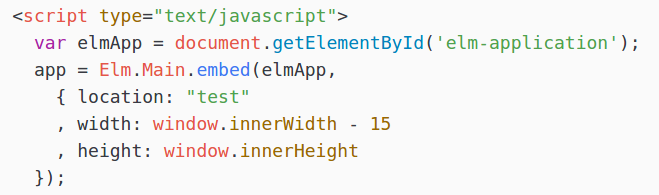
\includegraphics[scale=0.6]{img/programWithFlags_pass_data.png}
\caption{Eine beispielhafte Initialisierung der Elm-Applikation mit initialen, dynamischen Werten}\label{fig:programWithFlags}
\end{figure}
Die Abbildung~\ref{fig:programWithFlags} zeigt beispielhaft die Implementierung der $Html.App.programWithFlags$-Funktion. Der zweite Übergabeparameter an die $Elm.Main.embed$-Funktion ist dabei ein $Record$ mit den gewünschten initialen Werten.
Für die Umsetzung dieses praktischen Beispiels ist der Grundaufbau wie in Abbildung~\ref{fig:elm-grundaufbau-start} notwendig. Dies sind die minimal notwendigen Funktionen, um in den weiteren Schritten die einzelnen Sektionen des Views von \ac{HTML} nach Elm zu portieren, in einzelne Funktionen auszulagern und letzten Endes der Versuch, die gesamte Applikation zu modularisieren.
Aus der Abbildung~\ref{fig:elm-grundaufbau-start} wird ersichtlich, dass zunächst das gesamte Paket $elm-lang/html$ importiert wird. Die vorherige Installation des Pakets ist analog zu der in der Abbildung~\ref{fig:elm-install-package} beschriebene Vorgehensweise. Des Weiteren wird der Grundaufbau der Elm-Applikation ersichtlich.
Innerhalb der $main$-Funktion werden dabei alle notwendigen Funktionen an die $HTML$-Bibliothek weitergereicht. Dazu gehören die $init$, $view$, $update$ und $subscriptions$-Funktionen. Wie der Name bereits suggeriert initiiert die $init$-Funktion ein $Model$. Dabei wird dieses entweder anhand der dynamisch übergebenen Werte, oder durch ein Ausweich-Model ($initialModel$) erstellt, falls keine Daten übergeben wurden.
Die Funktion $view$ erzeugt in der Abbildung~\ref{fig:elm-grundaufbau-start} zunächst ein $div$-Element, während die $update$-Funktion auf jede eingehende Interaktion ein Tupel mit einem unveränderten $model$, sowie keinem $Effekt$ zurück gibt. Um die Applikation aufzurufen muss die Datei $index.html$ im Browser geöffnet werden.


\subsection{Überführung des Views}
\label{sec:ueberfuehrung-view}
Nachdem der Grundaufbau der Elm-Applikation beidseitig ausgeführt wurde, können nun die einzelnen Sektionen der originalen $index.html$ aus dem $Agency$-Template nativ in Elm überführt werden. Dafür wird das Online-Tool $html-to-elm$ auf der Webseite \url{http://mbylstra.github.io/html-to-elm/} zur Hilfe genommen. Der gesamte zuvor im $body$-Tag befindliche \ac{HTML}-Code wird kopiert und zur Konvertierung in das entsprechende Textfeld des Tools eingefügt. Der konvertierte Elm-Code sollte daraufhin auf der gegenüberliegenden Seite zu sehen sein. Durch einen Klick auf $copy$ wird der erstellte Elm-Code in die Zwischenablage kopiert, so dass der Inhalt in die $view$-Funktion der $Main.elm$-Datei eingefügt werden kann. Der kopierte Text fungiert dabei als kompletter Rückgabewert der $view$-Funktion.
\begin{figure}[h]
\centering
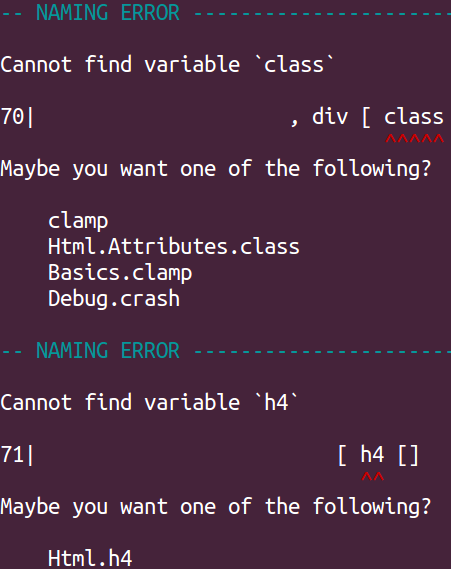
\includegraphics[scale=0.5]{img/elm-naming-error.png}
\caption{Elm-Compilerfehler bei fehlenden Funktionen im Namensraum}\label{fig:elm-naming-error}
\end{figure}
Das Tool $html-to-elm$ sollte den Code bereits nach den Regeln des Style-Guides formatiert haben, so dass hiermit der erste Schritt der Portierung abgeschlossen ist. Um Namenskonflikte im aktuellen Namensraum zwischen Funktionen zu verhindern, werden innerhalb der importierten $HTML$-Bibliothek die genutzten Funktionen zur Erstellung von \ac{HTML}-Code explizit genannt. Der Compiler sollte nach dem Entfernen des Kommandos $exposing (..)$ eine Warnung ausgeben und auf die fehlenden Funktionen hinweisen, wie es in Abbildung~\ref{fig:elm-naming-error} gezeigt wird. Schlägt der Compiler dabei vor, die Funktion aus dem Namensraum $Html.Attributes$ aufzurufen, muss sie entsprechend in die Liste der zu ladenden Funktionen der $Attribute$ hinzugefügt werden, wie in Abbildung~\ref{fig:elm-grundaufbau-start} in Zeile 3. Die Funktionen zur Generierung von \ac{HTML}-Tags hingegen sollten in die Liste der $import\,Html$s stehen. Nachdem alle Funktionen korrekt in den aktuellen Namensraum aufgenommen wurden, sollten keinerlei Compilerfehler auftreten.


\subsection{Beheben von JavaScript-Fehlern}
\label{sec:javascript-errors}
Das Öffnen der Seite mitsamt der Developer-Tools von Google-Chrome verrät, dass die bisher eingebundenen \ac{JS}-Dateien nicht fehlerfrei funktionieren. Nutzt man das Template wie vorgesehen, ist sämtliche Funktionalität vorhanden. Bei der Überführung des Templates in Elm gilt es allerdings zu beachten, dass die Elm-Applikation den $view$ ausliefert und diesen erst verzögert darstellt. Dem menschlichen Betrachter fällt dies zwar nicht auf, jedoch greifen die \ac{JS}-Skripte auf ein noch nicht geladenes Element zu. Es ist dementsprechend notwendig, die einzelnen Skripte anzupassen und mit Hilfe der $\$(document).ready()$-Funktion des Frameworks $jQuery$ (\url{https://learn.jquery.com/using-jquery-core/document-ready/}) erst nach dem kompletten Seitenaufbau zu laden.
Innerhalb der Datei $agency.js$ muss nicht nur die Funktion $\$('a.page-scroll').bind(...)$, sondern auch die nachfolgenden Funktionen innerhalb des $\$(function(){..});$-Blocks liegen. Die \ac{JS}-Datei $cbpAnimatedHeader.js$ hingegen erzeugt einen Fehler, wie in Abbildung~\ref{fig:js-classie-error} zu sehen ist.
\begin{figure}[h]
\centering
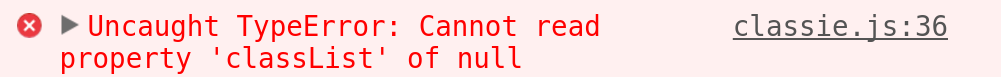
\includegraphics[scale=0.4]{img/error-javascript-classie.png}
\caption{JavaScript-Fehler innerhalb der Developer-Tools}\label{fig:js-classie-error}
\end{figure}
Um diesen zu beheben, muss der gesamte Dateiinhalt in eine $\$(document).ready()$-Funktion geschachtelt werden. Zusätzlich dazu ist es notwendig, dass die Codezeile wie sie in Abbildung~\ref{fig:code-to-add} zu sehen ist, als erstes in der Funktion $scrollPage()$ hinzugefügt wird.
\begin{figure}[h]
\centering
header = document.querySelector( '.navbar-fixed-top' );
\caption{Notwendiger Code, um JavaScript-Fehler zu beheben.}\label{fig:code-to-add}
\end{figure}
Der Code hat zur Folge, dass das Navigations-Element ausgewählt und an die $classie$-Funktion weitergegeben wird. Fehlt diese Zeile, erfolgt ein Aufruf der $classie$-Funktion mit einem undefinierten Wert, wodurch der Fehler in Abbildung~\ref{fig:js-classie-error} zustande kommt. Nachdem diese beiden Fehler behoben wurden, kann nun die $Scroll-Spy$-Funktionalität auf der Webseite betrachtet werden. Scrollt der Nutzer nun auf oder ab und befindet sich dabei in einer innerhalb der Navigation definierten Sektion, so wird das entsprechende Gegenstück in der Navigationsleiste farblich hinterlegt. Des Weiteren verkleinert sich die Navigationsleiste, wenn der Nutzer eine bestimmte Entfernung nach unten gescrollt hat.


\subsection{Auslagern des Views}
\label{sec:auslagern-des-views}
Um die einzelnen Sektionen der Webseite im Quellcode klar voneinander zu trennen, werden die einzelnen Sektionen in eine jeweils eigene Funktion ausgelagert.
Für jede Sektion wird hierfür eine gleichnamige Funktion angelegt, die dem Muster in Abbildung~\ref{fig:elm-view-section} folgt. Die $id$ eines \ac{HTML}-Elementes könnte entsprechend für den Funktionsnamen $nameDerSektion$ genutzt werden, da dieses Attribut ohnehin einzigartig in einem gesamten \ac{HTML}-Dokument vorkommt und eine klare Namensgebung liefert.
\begin{figure}[htb]
\centering
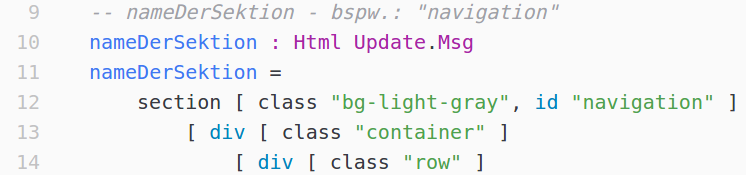
\includegraphics[scale=0.53]{img/elm-html-sections.png}
\caption{Deklaration einer Sektion des Views in Elm}\label{fig:elm-view-section}
\end{figure}
Am Beispiel der $portfolio$-Sektion des zu überführenden Templates sehen die daraus resultierende Funktion teilweise aus wie in Abbildung~\ref{fig:elm-view-section-function}. Die einzelnen Klassen und ID`s wurden beibehalten und übernommen. Nachdem die einzelnen Sektionen in Funktionen ausgelagert wurden fällt auf, dass die Sektionen nicht mehr angezeigt werden. Dafür ist es notwendig die ursprüngliche $view$-Funktion mit den Funktionsaufrufen der Sektionen zu versehen. Dieses Vorgehen kann in der Abbildung ~\ref{fig:elm-view-sections-call} betrachtet werden. Das Resultat der $view$-Funktion unverändert aus, ist jedoch nun im Code übersichtlicher.
\begin{figure}[h]
\centering
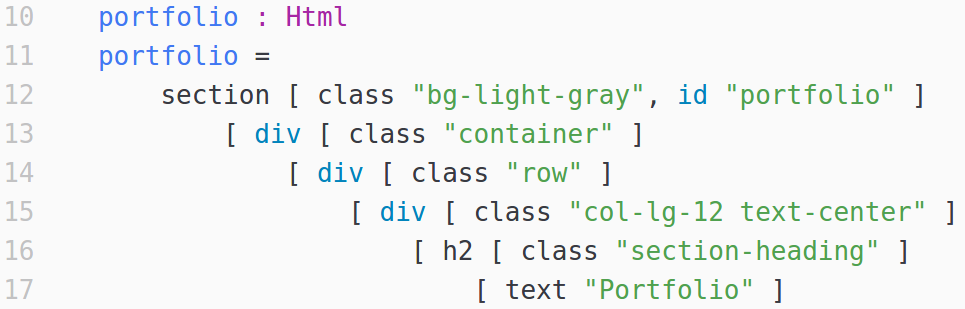
\includegraphics[scale=0.41]{img/elm-view-portfolio-section-function.png}
\caption{Ausgelagerter View in eine eigene Funktion}\label{fig:elm-view-section-function}
\end{figure}

\begin{figure}[h]
\centering
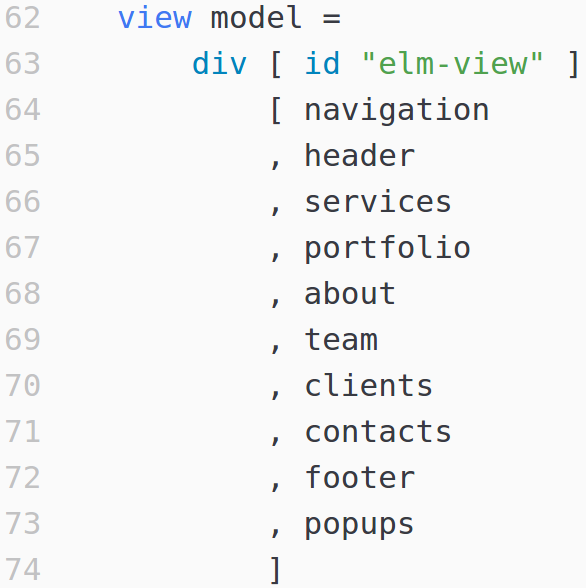
\includegraphics[scale=0.4]{img/elm-view-section-functions-calling.png}
\caption{Aufruf der einzelnen Sektionen im View}\label{fig:elm-view-sections-call}
\end{figure}


\subsection{Hinzufügen von Klick-Events}
\label{sec:erweiterung-clicks}
Der derzeitige Stand der überführten Applikation stellt bereits sämtliche Sektionen auf der Webseite dar und erlaubt das Öffnen eines Modals durch einen Klick auf eines der Portfolio-Elemente. Bei einem Klick auf ein Element in der Navigationsleiste springt der Viewport des Browsers jedoch ohne jegliche Verzögerung direkt auf die ausgewählte Sektion. Das ursprüngliche Template hingegen nutzt die Funktionalität $smooth-page-scrolling$, wodurch der Nutzer einen sichtbaren Scroll-Effekt erhält, während automatisch zur ausgewählten Sektion gescrollt wird. Innerhalb der Datei $agency.js$, in der vorab bereits die Funktion des $Scroll-Spy$s wiederhergestellt wurde, wird in den Zeilen $9$ bis $15$ die Funktionalität des automatischen scrollens bei einem Klick umgesetzt, wie in Abbildung~\ref{fig:non-functional-scrolling} zu sehen ist.
\begin{figure}[h]
\centering
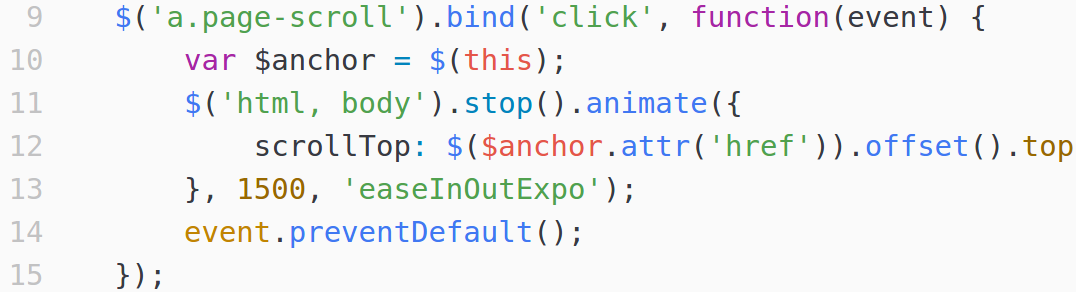
\includegraphics[scale=0.37]{img/non-functional-scrolling}
\caption{Funktion zum scrollen bei einem Klick}\label{fig:non-functional-scrolling}
\end{figure}
Dabei wird zunächst ein $Ereignisbehandler$ an die Link-Elemente mit der Klasse $page-scroll$ gebunden. Klickt der Nutzer eines dieser Elemente, so wird die darauf folgende Funktion ausgeführt. Diese Funktion wiederum ließt Informationen des angeklickten Elementes aus, insbesondere das $href$-Attribut, welches die Id zur angeklickten Sektion enthält. Mittels der $animate$-Funktion wird letztlich zur gewünschten Sektion gescrollt.
Diese Funktionalität ist nicht verfügbar, da das externe \ac{JS} versucht auf \ac{HTML}-Elemente innerhalb der Elm-Applikation zuzugreifen. Um dieses Problem zu lösen, kann einerseits die Funktion innerhalb der Datei $agency.js$ umgeschrieben werden, so dass sämtliche Klicks innerhalb des $body$-Elementes abgefangen werden, da sich dieser nicht Teil der Elm-Applikation ist. Andererseits kann der Klick innerhalb der Elm-Applikation registiert und über sogenannte Ports nach außen getragen werden. In diesem Beispiel ist das die bevorzugte Methode, da so eine klare Trennung zwischen der Elm-Applikation und den externen \ac{JS}-Skripten herrscht.
Die Elm-Bibliothek $Html.Events$ enthält die Methode $onWithOptions$, mit Hilfe derer ein Klick auf ein Element des $views$ in Elm eine $Msg$ erzeugt. Diese $Msg$ wird an die $update$-Funktion weitergeleitet und kann dort entsprechend ausgewertet werden.
\begin{figure}[htb]
\centering
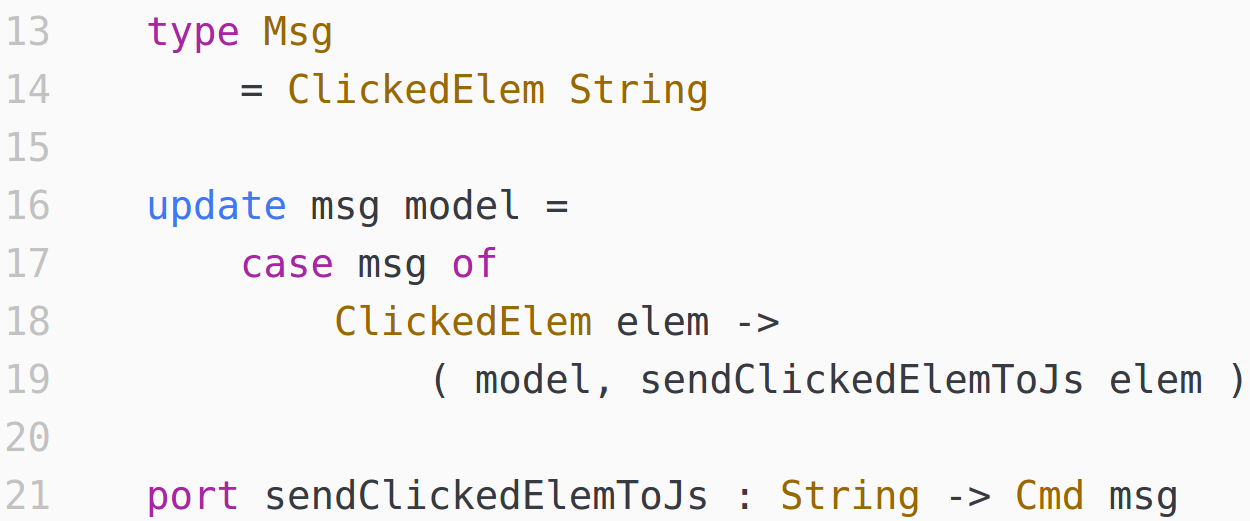
\includegraphics[scale=0.3]{img/elm-port.png}
\caption{Definition eines neuen Union Types, sowie eines Ports für die Kommunikation zwischen Elm und \ac{JS}}\label{fig:create-port}
\end{figure}
Bislang gibt es in der Elm-Applikation noch keine $Msg$-Typen, welche die $update$-Funktion verarbeiten könnte. Dementsprechend wird zunächst ein neuer Union-Type $Msg$ mit dem Eintrag $ClickedElem\,String$ angelegt. Der Union-Type muss nun noch in der $update$-Funktion behandelt werden. Hierbei wird ein neuer $case$ angelegt, mit dem zuvor erstellten Eintrag $ClickedElem$ und dem Übergabeparameter $elem$ vom Typ $String$. Der vorherige Eintrag "$\_ ->$", welcher für alle Fälle gilt, kann entfernt werden. Der Rückgabewert des $ClickedElem$-Falles ist dabei ein Tupel, bestehend aus dem unveränderten $model$, sowie einem Effekt. In diesem Fall ist der Effekt das Senden der ausgewählten Elemente nach außen zu einem \ac{JS}-Skript, das die Daten verarbeitet. Der Effekt wird dabei über den Port $sendClickedElemToJs$ nach außen geschickt. Der Port muss definiert werden mit dem Kommando in Zeile $21$ aus der Abbildung~\ref{fig:create-port}. Das Kommando ist lediglich die Signatur der gewünschten Kommunikationsweise und wird durch den Elm-Compiler während des Kompiliervorgangs entsprechend verarbeitet.
Beim Versuch den Code wie er in Abbildung~\ref{fig:create-port} zu sehen ist zu kompilieren, wird der Compiler mit der Fehlermeldung "You are declaring port $sendClickedElemToJs$ in a normal module" antworten. Die Fehlermeldung bedeutet, dass das Modul in dem ein Port definiert wird explizit als ein Port-Modul deklariert werden muss. Die erste Zeile des Hauptmoduls muss folglich noch mit dem Schlüsselwort $port$ versehen werden. Damit die Elm-Applikation die Funktion $ClickElem$ aufruft, bedarf es noch des Aufrufes der zuvor erwähnten $onWithOptions$-Methode. Diese wird in den $view$ an den entsprechenden Stellen eingesetzt. Die Links der Navigationsleiste befinden sich in der Funktion $navigation$ und müssen um den Zusatz der $onWithOptions$-Funktion, sowie den Übergabeparametern $ClickedElem$ und dem $href$-Wert erweitert werden. In Abbildung~\ref{fig:elm-view-onclick} kann beispielhaft die Erweiterung an einigen Stellen begutachtet werden. Die Funktion $onWithOptions$ bekommt dabei zunächst einmal das $Event$, auf das sie einen Ereignishandler setzen soll. In diesem Fall ist dies ein $click$. Darauf folgt ein optionaler $Record$ von Typ $Options$. Hier müssen die Werte $stopPropagation$ und $preventDefault$ auf $True$ gesetzt werden. Fehlt diese Einstellung, so wird das scrollen sofort ausgeführt und kann möglicherweise andere Ergebnisbehandler in denen der Link geschachtelt ist ausführen. Dies würde zu einem undefinierten Verhalten führen. Der letzte Parameter ist die die Decoder-Funktion $Json.succeed$. Sie führt dazu, dass die übergebene Funktion $ClickedElem$ direkt und ohne weitere Überprüfungen ausgeführt wird.
\begin{figure}[hbt]
\centering
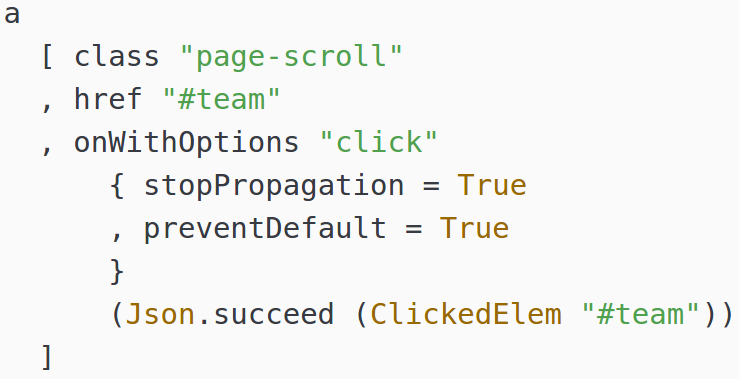
\includegraphics[scale=0.4]{img/elm-view-onclick.png}
\caption{Erweiterung des Views um einen $onWithOptions$ Ereignisbehandler in Elm}\label{fig:elm-view-onclick}
\end{figure}
Seitens der Elm-Applikation ist die notwendige Erweiterung nun abgeschlossen. Jedoch muss noch die $index.html$ um eine sogenannte $subscription$ erweitert werden. Das bedeutet, dass innerhalb der $index$-Datei die Nachricht der Elm-Applikation des angeklickten Elements entgegengenommen und verarbeitet werden muss. Diesbezüglich wird in der $index.html$ nach der Codestelle die für die Initialisierung der Elm-Applikation zuständig ist die Funktion aus Abbildung~\ref{fig:scrollTop} hinzugefügt.
\begin{figure}[hbt]
\centering
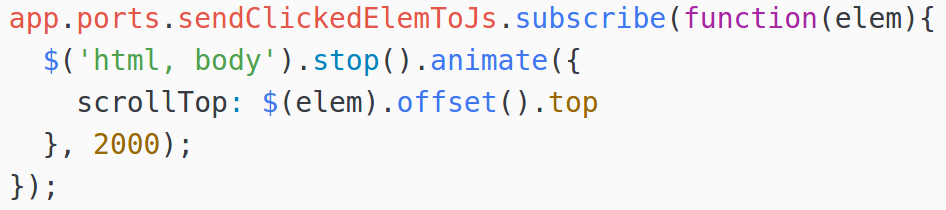
\includegraphics[scale=0.4]{img/scrollTop.png}
\caption{Entgegennahme der Daten aus der Elm-Applikation und anschließendes scrollen}\label{fig:scrollTop}
\end{figure}
Durch das Kommando $app.ports.sendClickedElemToJs.subscribe$ werden sämtliche Daten die Elm über den Port $sendClickedElemToJs$ sendet entgegengenommen und die nachfolgende Funktion ausgeführt. Diese Funktion wurde in diesem Beispiel lediglich aus der Datei $agency.js$ kopiert. Sie ermittelt das \ac{HTML}-Element im Baum anhand der übergebenen Id und scrollt innerhalb von zwei Sekunden zur obersten Stelle des übergebenen Elements.

\subsection{Modularisierung der Applikation}
\label{sec:modularisierung-der-applikation}
Durch das Auslagern aller einzelnen Sektionen der darzustellenden \ac{HTML}-Elemente ist die daraus resultierende $Main.elm$-Datei recht unübersichtlich. Abhängigkeiten zwischen einzelnen Funktionen sind kaum mehr erkennbar und die Programmlogik ist nicht unterscheidbar von Funktionen, die für die Darstellung des Views zuständlich sind. Folglich ist es sinnvoll einzelne Teile der Applikation in mehrere Dateien und Ordner zu verschieben. Eine solche Strukturierung hilft dabei, die womöglich fehlerbehafteten Teile der Applikation schneller zu finden und die einzelnen Bereiche der Applikation deutlicher voneinander zu trennen. Dabei werden die einzelnen Programmteile des Views ausgelagert in eigene Module. Dasselbe Prinzip wird für das Model und die Update-Funktion angewandt. Im Gegenzug sollen die ausgelagerten Programmteile global im Hauptmodul importiert und an den entsprechenden Stellen aufgerufen werden.

\subsubsection{View}
\label{sec:auslagern-view}
Jede Funktion die bisher eine Sektion des Views erzeugt hat, wird in eine neu angelegte $.elm$-Datei verschoben und die Funktion umbenannt zu $view$. Die Datei bekommt dabei den Namen, den die Funktion vorher trug. Ferner wird ein Ordner $View$ erzeugt, in den all diese Dateien hin verschoben werden. Damit die neuen Dateien als Module eingebunden werden können, müssen sie als solches definiert werden. Das bedeutet, dass jede Datei mit dem Kommando $module\,View.NameDerDatei\,exposing\,(view)$ initialisiert werden muss. Der Zusatz $view$ nach dem Kommando $exposing$ gibt an, dass die Funktion $view$ nach außen hin sichtbar ist und vom importierenden Modul genutzt werden kann.
\begin{figure}[hbt]
\centering
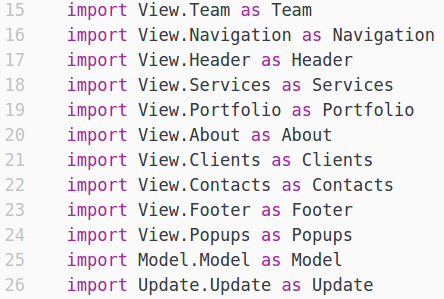
\includegraphics[scale=0.5]{img/imports-main.png}
\caption{Einbindung und Aufruf der ausgelagerten View-Funktionen}\label{fig:elm-main-view-imports}
\end{figure}
Nachdem alle Funktionen in ein eigenes Modul ausgelagert wurden, müssen alle Module im Hauptmodul $Main.elm$ importiert werden. Des Weiteren müssen die $view$-Funktionen der einzelnen Module im Hauptmodul aufgerufen werden. Die Abbildungen~\ref{fig:elm-main-view} und \ref{fig:elm-main-view-imports} zeigen die $view$-Funktion des Hauptmoduls, sowie den Aufruf um die angelegten Module zu importieren.
\begin{figure}[hbt]
\centering
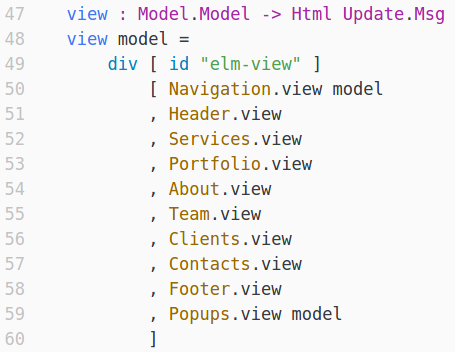
\includegraphics[scale=0.6]{img/view-main.png}
\caption{Einbindung und Aufruf der ausgelagerten View-Funktionen}\label{fig:elm-main-view}
\end{figure}
Letzten Endes müssen die einzelnen Module noch mit den notwendigen $import$s für die verwendeten Funktionen erweitert werden. Das Hauptmodul wiederum kann von den nicht benutzten $Html$- beziehungsweise $Html.Attributes$-Funktionen gesäubert werden.

\subsubsection{Update}
\label{sec:auslagern-update}
Nicht nur die für die Darstellung verantwortlichen Funktionen sollten modularisiert werden, sondern auch die Programmlogik. Hierfür wird ein weiterer Ordner $Update$ erzeugt. Die bisherige $update$-Funktion wird demzufolge analog zu den $View$-Funktionen ausgelagert in ein eigenes Modul im neu erzeugten Ordner $Update$. Das $Update$-Modul folgt derselben Namensgebung wie ein einzelner $View$ und wird definiert als $Update.Update$. Zusätzlich müssen auch an dieser Stelle die $import$s der benutzten Pakete übernommen und definiert werden, wobei das Hauptmodul diese entfernen kann.

\subsubsection{Model}
\label{sec:auslagern-Model}
Letztlich wird noch das $model$, das sämtliche Daten die den Status der Applikation beschreiben enthält, in ein eigenes Modul im Unterordner $Model$ überführt. Die Einbindung dieses Moduls funktioniert analog zur Modularisierung von $Update$ und $View$.
Mit Hilfe dieser Modularisierung wird das angestrebte \ac{MVU}-Konzept von Elm besonders deutlich.


\subsubsection{Asynchrones Laden von Daten}
\label{sec:async-laden}
Klickt man innerhalb der Portfolio-Sektion der Webseite auf ein Element, öffnet sich ein Modal in dem weitere Informationen dargestellt werden. Die bestehende Elm-Applikation wird nun um das Feature des asynchronen Ladens von Informationen erweitert, die anschließend in dem geöffneten Modal angezeigt werden. Beispielhaft wird hier die \ac{API} von \ac{ICNDb} (\url{https://api.icndb.com}) genutzt. Sie liefert bei jeder Anfrage einen zufälligen Witz zurück.
Für dieses Funktionalität muss zunächst das $model$ erweitert und angepasst werden, da dies die einzige Möglichkeit in einer Elm-Applikation ist, Daten beziehungsweise den Status der Applikation zu speichern. Das $model$ bekommt entsprechend ein weiteres Feld $async\_content$ vom Typ $String$.
Bei einem Klick auf einen der Portfoliobeiträge soll ein Modal geöffnet und ein zufälliger Witz präsentiert werden. Dafür wird über die externe \ac{API} ein zufälliger String angefordert, vom Server generiert und letztlich an die Elm-Applikation zurückgegeben. Ebenso wäre es möglich einen Server für das Backend zu erstellen, auf dem eine Datenbank läuft, so dass Daten asynchron angefordert werden können. Das asynchrone Anfordern von Daten basiert sowohl bei einem lokalen, wie auch externen Server auf dem gleichen Konzept, weswegen dieser Schritt entfällt und der vorhandene externe Service genutzt wird.
Ein solcher asynchroner Request stellt im Grunde eine Verletzung des Konzeptes von Elm dar, dass es keinerlei Seiteneffekte gibt. Da nicht bekannt ist, wann der Request endet und welchen Status die Antwort besitzt, ist zunächst nicht vorhersehbar, wie der Status der Applikation nach dem Request aussehen wird. Um dieses Problem zu vermeiden, ist es notwendig alle möglichen Fälle, sprich den Fall einer erfolgreichen, sowie fehlerhaften Übertragung, zu behandeln. Auf diese Weise ist gewährleistet, dass die Applikation sich nicht plötzlich in einem undefinierten Zustand befindet. Es bedarf zusätzlich der Bibliotheken $Http$, $Json.Decode$ und $Task$, damit ein asynchroner Request ausgeführt werden kann. Die Bibliotheken müssen installiert und in die jeweiligen Module importiert werden. Des Weiteren gilt es den Klick auf den Portfoliobeitrag abzufangen, um den Request zu starten und das Ergebnis in den View einzuarbeiten. Dafür gibt es die $onClick$ Funktion aus der $Html.Events$-Bibliothek. Sie bekommt eine auszuführende Funktion aus dem $Update$-Modul als Parameter, in diesem Fall $GetRandomString$, wie es in Abbildung~\ref{fig:portfolio-async} zu sehen ist. Bei einem Klick auf das Element wird eine $Msg$ von diesem Typ erstellt und muss in der $update$-Funktion behandelt werden.
\begin{figure}[h]
\centering
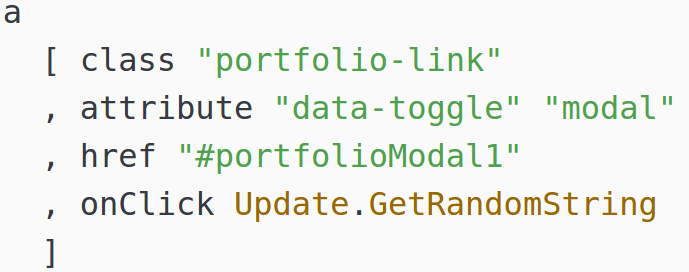
\includegraphics[scale=0.4]{img/portfolio-async.png}
\caption{OnClick-Ereignisbehandler in Elm}\label{fig:portfolio-async}
\end{figure}
Wie zuvor bei der Definition einer $Msg$ um Daten durch Ports nach außen zu kommunizieren, muss auch die Nachricht $GetRandomString$ als $Msg$-Typ deklariert werden, um so in der $update$-Funktion behandelt werden zu können. Außerdem müssen die möglichen Statusfälle des Requests behandelt und als $Msg$ hinzugefügt werden. Abbildung~\ref{fig:msg-async} zeigt die hinzugefügten $Msg$-Typen.
\begin{figure}[h]
\centering
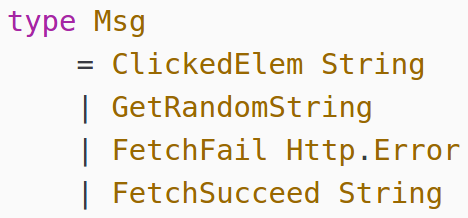
\includegraphics[scale=0.5]{img/msg-async.png}
\caption{$Msg$-Deklaration mit asynchronem Request}\label{fig:msg-async}
\end{figure}
Nachdem die neuen Interaktionsmöglichkeiten in der Elm-Applikation implementiert wurden, muss nun der eigentliche Request ausführbar gemacht werden. Die Funktion $GetRandomString$ soll dabei ein unverändertes Model, sowie eine asynchron auszuführende Funktion in Form eines Effektes als Tupel zurückliefern. Dabei ist die asynchrone Funktion der eigentliche \ac{HTTP}-Request, wie er in Abbildung~\ref{fig:fetchasync-async} erkennbar ist.
\begin{figure}[h]
\centering
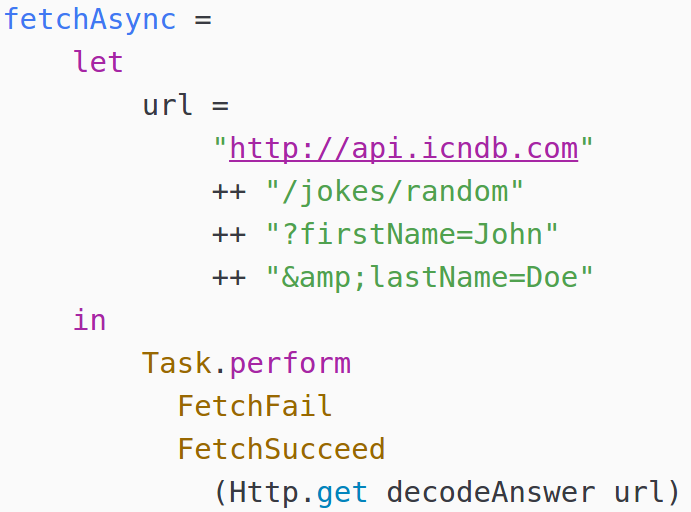
\includegraphics[scale=0.3]{img/fetchasync-async.png}
\caption{Asynchroner \ac{HTTP}-Request in Elm}\label{fig:fetchasync-async}
\end{figure}
Dabei wird die Funktion $Http.get$ genutzt, um einen Request an die $url$ auszuführen. Die Antwort des Requests wird an die Funktion $decodeAnswer$ gereicht, welche das eingehende \ac{JSON}-Objekt dekodiert und die gewünschten Informationen herausfiltert. Die Dekodierfunktion kann in Abbildung~\ref{fig:decodeanswer-async} betrachtet werden. Sie filtert das geschachtelte \ac{JSON}-Objekt, so dass nur der gewünschte String übrig bleibt.
\begin{figure}[h]
\centering
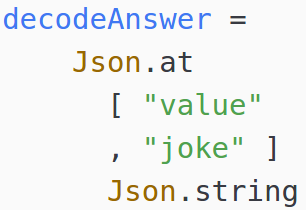
\includegraphics[scale=0.4]{img/decodeanswer-async.png}
\caption{Dekodierung eines Json-Objektes in Elm}\label{fig:decodeanswer-async}
\end{figure}
Abhängig vom Status des Requests, wird der jeweilige Fall in der $update$-Funktion aufgerufen. Bei einer erfolgreichen Übertragung wird die Funktion $FetchSucceed$ ein neues Model mit dem asynchron abgerufenen String zurückliefern. Der String wird dabei in das Feld $async\_content$ des $model$ geschrieben. Bei einer fehlgeschlagenen Übertragung wird die Funktion $FetchFail$ das unveränderte $model$ zurückgeben. Alternativ kann auch eine mögliche Fehlermeldung in das $model$ eingearbeitet und im $view$ dargestellt werden.
\begin{figure}[h]
\centering
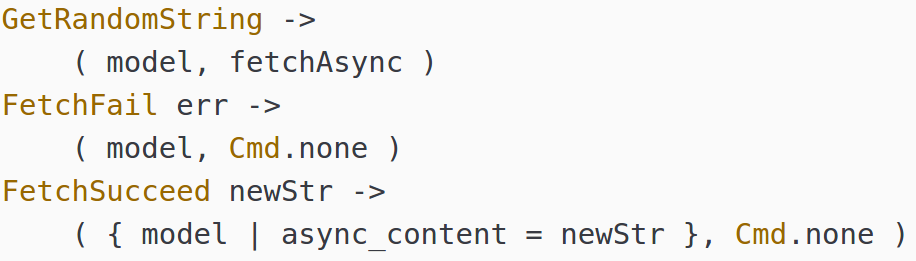
\includegraphics[scale=0.4]{img/update-async.png}
\caption{$Update$-Fälle für den asynchronen Request}\label{fig:update-async}
\end{figure}
Die fertige $update$-Funktion mit allen abgehandelten Fällen ist in Abbildung~\ref{fig:update-async} dargestellt. Der asynchrone Request wird dabei durch $GetRandomString$ initiiert. Die Manipulation des $model$ findet lediglich in der $FetchSucceed$-Funktion statt.
Nachdem die Elm-Applikation an dieser Stelle fehlerfrei kompiliert wurde, kann der asynchrone Request auf der Webseite getestet werden. Mit Hilfe der Developer-Tools kann die ausgehende Anfrage an den \ac{ICNDb}-Server beobachtet und ausgewertet werden. Auch die Antwort des Servers kann unbehandelt in Abbildung~\ref{fig:request-async} begutachtet werden.
\begin{figure}[htb]
\centering
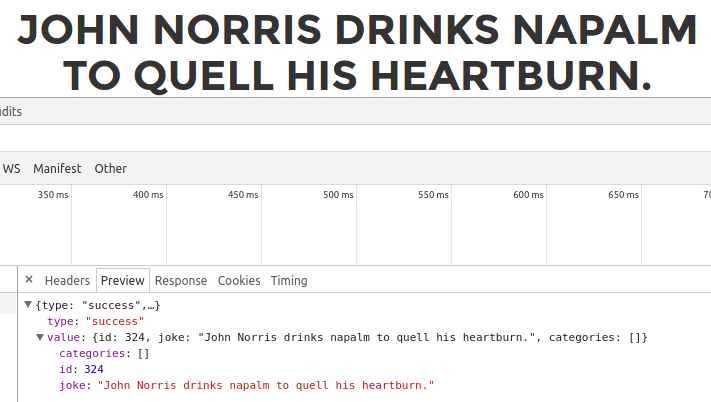
\includegraphics[scale=0.4]{img/request-async.png}
\caption{Ausgehender HTTP-Request und eingehende Antwort}\label{fig:request-async}
\end{figure}
Die Abbildung zeigt ferner wie der zurückgelieferte Text des Requests fehlerfrei dekodiert und in das $model$ übertragen, sowie letztlich in der $view$-Funktion des $Popup$-Moduls mittels des Kommandos $text\,model.async\_content$ angezeigt wird.



\subsection{Beobachtungen}
\label{sec:Beobachtungen}
In diesem Abschnitt sollen Auffälligkeiten, die während der Überführung des $agency$-Templates in eine native Elm-Applikation auftraten, aufgezeigt und erläutert werden. Es handelt sich hierbei nicht nur um Probleme, sondern auch um interessante Erkenntnisse im Hinblick auf die Unterschiede zwischen herkömmlicher Webentwicklung mit \ac{HTML}, \ac{CSS} und \ac{JS} gegenüber Elm, die es zu erwähnen gilt.

\subsubsection{Natives Einbinden von CSS in Elm nur beschränkt möglich}
Herkömmlicherweise können Elemente einer \ac{HTML}-Datei auf drei Arten gestylt werden.
\begin{enumerate}
\item{Inline \ac{CSS}:}
	\subitem Das Inline \ac{CSS} erlaubt Design-Anpassungen für genau ein bestimmtes Element. Der verfasste \ac{CSS}-Code kann nicht von anderen Elementen genutzt werden und wird über das \ac{HTML}-Attribut $style$ eingeführt.
\item{Internes \ac{CSS}:}
	\subitem \ac{HTML} enthält den $style$-Tag. In diesem kann natives \ac{CSS} verfasst, bestimmte Klassen oder Id's erstellt und sämtliche gängigen Design-Anpassungen durchgeführt werden.
\item{Externes \ac{CSS}:}
	\subitem Die Erweiterung des internen \ac{CSS} ist das externe \ac{CSS}, bei dem der gesamte \ac{CSS}-Code ausgelagert wird in eine eigene $.css$-Datei. Diese wird wiederum mit Hilfe des $link$-Tag der \ac{HTML}-Datei eingebunden.
\end{enumerate}
In Elm ist es nicht möglich nativen \ac{CSS}-Code zu verfassen. Jedoch kann mittels der Bibliothek $elm-lang/html$ inline \ac{CSS} erzeugt werden. Das Design wird dabei nativ in Elm über die $Html.style$-Funktion programmiert. Ferner ist das erstellen von $style$-Tags in Elm nicht möglich, wodurch auch die Möglichkeit für internes \ac{CSS} entfällt. Es ist zwar praktisch möglich externe \ac{CSS}-Dateien in die Elm-Applikation nativ in Elm einzubinden, jedoch stört das immens die Nutzbarkeit der Applikation. Die Elm-Applikation wird zunächst ohne das \ac{CSS} geladen, während die externe Datei nachgeladen wird. Das bedeutet für den Nutzer der Webseite, dass zunächst nur Texte und Bilder ohne Styling angezeigt werden. Nachdem die externe Datei vollständig übertragen wurde, wird das darin enthaltene Design auf die \ac{HTML}-Elemente angewandt. Der zeitliche Abstand zwischen initialem Laden und der Anwendung des Stylesheets hat ein sichtbares $flackern$ zur Folge, wodurch eine Nutzung in einem fertigen System entfällt. Dies ist der Grund, weswegen bereits bestehende \ac{CSS}-Dateien des Templates nicht nativ in Elm überführt, sondern über das \ac{HTML}-Grundgerüst eingebunden wurden. Zusätzlich zu diesem Umstand wird inline- und internes \ac{CSS} nicht vom Browser zwischengespeichert. Das hat eine längere Ladezeit zur Folge und sollte vermieden werden. Des Weiteren ist es nur bedingt möglich \ac{CSS}-Code in Elm an mehreren Stellen zu verwenden, wie es üblicherweise mit in \ac{CSS} definierten Klassen der Fall ist.


\subsubsection{HTML-Code ist in Elm wesentlich kürzer}
\ac{HTML}-Tags mit den gleichnamigen Funktionen nativ in Elm zu erstellen ist einerseits signifikant kürzer, andererseits viel übersichtlicher als das Verfassen von herkömmlichen \ac{HTML}-Code.
\begin{figure}[h]
\centering
HTML:
<div>
</div>\\
Elm:
div[$\,$][$\,$]
\caption{Ein $div$-Element in \ac{HTML} und Elm}\label{fig:div-element}
\end{figure}
Die Abbildung~\ref{fig:div-element} zeigt ein $div$-Element, wie es einerseits in klassischem \ac{HTML}, andererseits in Elm realisiert wird. In Elm handelt es sich dabei um einen Funktionsaufruf mit zwei Parametern, in diesem Fall zwei leeren Listen. Ein \ac{HTML}-Element hat dabei eine Anzahl von $5+2*n_0$ Zeichen, wobei $n_0$ gleich der Zeichenanzahl des Tag-Namens und $5$ die Zeichen für das öffnende, sowie schließende Tag sind. Am Beispiel des $div$-Elementes wäre $n_0:=3$, wodurch die Implementierung in \ac{HTML} $5+2*3$, sprich $11$ Zeichen benötigt.
In Elm hingegen benötigt die Erstellung eines \ac{HTML}-Elementes $4+n_1$ Zeichen, wobei $n_1$ gleich der Zeichenanzahl des Tags, sprich hier der Funktion $div$, und $4$ die Zeichenanzahl für die Parameterliste ist. Am selben Beispiel wären das $4+3$, sprich $7$ Zeichen. Die Konstanten $5$ (\ac{HTML}) und $4$ (Elm) können vernachlässigt werden, wodurch sich die dynamischen Werte $2*n_0$ und $n_1$ gegenüberstehen. Da alle \ac{HTML}-Tags in Elm mit einer gleichnamigen Funktion erstellt werden, kann $n_0$ gleich $n_1$ gestellt werden. Daraus folgt, dass Elm im Vergleich zu \ac{HTML} 50\% weniger Zeichen für die Erstellung eines \ac{HTML}-Elementes benötigt.
Die Differenz der Zeichen lässt sich auf das schließen der Tags in \ac{HTML} zurückführen. Nativer Elm-Code arbeitet mit Einrückungen, wohingegen klassischer \ac{HTML}-Code über die öffnenden und schließenden Tags geschachtelt wird. Dadurch entsteht bei \ac{HTML}-Code der Vorteil, dass ein gesamtes Dokument theoretisch in nur einer Zeile ohne Absätze definiert werden kann, während in Elm die Einrückungen und die damit verbundenen Zeilenumbrüche notwendig sind. Daraus folgt, dass Elm-Code zwangsweise übersichtlicher bleibt, da die Einrückungen nicht umgangen werden können und dem Entwickler eine visuelle Rückmeldung liefern. Der Elm-Compiler wird den Elm-Code nicht in \ac{JS}-Code umwandeln, sollten die Abstände inkorrekt sein. \ac{HTML}-Code bietet die Möglichkeit gleichermaßen übersichtlich zu programmieren, jedoch gibt es hier keinen Compiler oder sonstige Warnhinweise für den Fall, dass geschriebener Code unübersichtlich wird.
Durch die Einrückung in das damit verbundene Fehlen von schließenden Tags kam es zu weniger Flüchtigkeitsfehlern in Form von falschen Verschachtelungen oder dem simplen Fehlen der schließenden Tags bei einer tiefen oder über mehrere Absätze stattfindende Schachtelung.

\subsubsection{Elm hat eine stark wachsende Open-Source Gemeinschaft}
Trotzdem Elm erst im März 2012 entwickelt wurde, gibt es bereits eine Vielzahl an Gemeinschaften, um über die Sprache zu diskutieren, Hilfe zu erbitten oder gemeinsam an Projekten zu arbeiten. Neben einem eigenen Slack-Chatroom mit 2.701 angemeldeten Nutzern \cite[vgl.]{slack-user}, gibt es noch die offizielle Google-Gruppe. Offiziell gibt es derzeit $205$ Elm-Bibiliotheken \cite[vgl.]{elm-package}, von denen jede einzelne ein Open-Source-Projekt darstellt und für alle Entwickler freigegeben ist. Auf der Webseite \url{https://github.com/} gibt es zur Zeit 2.845 öffentliche Projekte \cite[vgl.]{elm-repositories} die in, oder mit Elm realisiert wurden. Ferner wurden 6.365 Probleme in diesen Projekten gemeldet, von denen 4.834 bereits gelöst und 1.531 noch geöffnet sind.  Alles in Allem wird deutlich, dass Elm eine wachsende Anhängerschaft besitzt und die Probleme der Webentwicklung auf eine andere Weise angeht. Wann immer Fragen auftraten konnten die Nutzer in einem der genannten Medium meist in wenigen Minuten aushelfen. War dies nicht der Fall, wurden stets weitere Nutzer kontaktiert, bis das Problem endgültig gelöst wurde.



%\begin{enumerate}[label*=\arabic*.]
%
%\item Externes \ac{CSS} kann nicht nativ über Elm geladen werden
%	\begin{enumerate}[label*=\arabic*.]
%		\item Inline-\ac{CSS} muss manuell mehrfach abgeändert werden
%		\item Keine Schachtelung möglich
%		\item Browser kann inline-\ac{CSS} nicht zwischenspeichern
%	\end{enumerate}
%\item Ein \ac{HTML}-Element benötigt in Elm weniger Zeichen
%	\begin{enumerate}[label*=\arabic*.]
%		\item \ac{HTML}-Code benötigt in Elm keine schließenden Klammern. Anders als \ac{HTML} arbeitet Elm mit Einrückungen. Die gleichnamigen Funktionen um ein \ac{HTML}-Element zu erzeugen benötigen dementsprechend lediglich den Funktionsaufruf, gefolgt von den zwei Argumenten. Das bedeutet, dass nativer Code in Elm kürzer und weniger anfällig für Flüchtigkeitsfehler wie beispielsweise das Schließen eines Tags ist. Der Entwickler wird weniger syntaktische Fehler machen.
%	\end{enumerate}
%\item Vertikale und horizontale Zentrierung eines Elementes ist umfangreicher als vorerst erwartet
%	\begin{enumerate}[label*=\arabic*.]
%		\item Obwohl Elm ein Paket für genau dieses Anwendungsgebiet besitzt, ist die Anwendung dennoch weder simpel, noch voll funktionsfähig. Es bedarf einiger Transformationen der Elemente, um sie in nutzbare, validen \ac{HTML}-Code zu formatieren. Zuletzt trifft der Entwickler auf die Problematik, zusätzlich noch die explizite Größe des Fensters mit einbeziehen zu wollen, so dass das Element den gesamten Bildschirm ausfüllt und einen zentrierten Text beinhaltet. Die Fenstergröße zu ermitteln stellt ein größeres Hindernis dar, als zunächst erwartet. Die Möglichkeiten sind hier, halbwegs dynamisch die Fenstergröße bei der Initiierung der Elm-Applikation an diese weiter zureichen, oder über Ports abzufangen, wenn sich die Fenstergröße geändert hat. Die erste Lösung hilft nur, wenn die Größe des Fensters nicht weiter verändert wird. Dies kann jedoch nicht gewährleistet werden, wodurch die Lösung entfällt. Die zweite Lösung hingegen erzeugt eine zusätzliche Abhängigkeit zwischen Elm und externem \ac{JS}. Zuletzt bleibt noch die altbekannte Möglichkeit mittels \ac{CSS} den Text in einem Element beidseitig zu zentrieren. Hierfür kann das externe \ac{CSS}-Framework Flexbox zuhilfe gezogen werden. Flexbox kümmert sich um die horizontale und vertikale Platzierung von Elementen, ohne auf die \ac{CSS}-Eigenschaft „float“ zurückgreifen zu müssen, die gerade bei tief verschachtelten Elementen Probleme verursacht.
%		
%		\item Das Paket `elm-lang/window` stellt eine Funktion `resize` zur Verfügung, die bei jeder Veränderung der Fensterdimensionen über eine sogenannte `subscription` in Elm einen Aufruf der `update` Funktion auslöst, an jene die neuen Fensterdimensionen (X, Y) weitergereicht werden.
%	\end{enumerate}
%
%\item Elm-Compiler
%	\begin{enumerate}[label*=\arabic*.]
%		\item Kompiliert abhängig von der Tiefe der Elemente
%		\begin{enumerate}[label*=\arabic*.]
%			\item Entwickler muss lesbaren Code erzeugen, da Elm sensitiv auf Tabs reagiert (vs\ac{HTML}: $<div><span></span></div>$ wo unendliches verschachteln auch in einer Zeile möglich ist)
%		\end{enumerate}
%	\end{enumerate}
%
%\item TODO:
%	\begin{enumerate}[label*=\arabic*.]
%		\item Fehlende Beispiele importieren
%		\item Umschreiben der Beispiele
%	\end{enumerate}
%\end{enumerate}


%
%\subsection{Hypothesen und Vermutungen}
%\label{sec:Hypothesen und Vermutungen}
%Sämtliche Hypothesen wurden in der Tabelle~\ref{tab:Hypothesentabelle} zusammengefasst. Dabei beziehen sich die einzelnen Vermutungen jeweils auf eines der zuvor erläuterten Kriterien in den Kapiteln \nameref{sec:Bewertungskriterien} (\ref{sec:Bewertungskriterien}) und \nameref{sec:ansprueche-webapp} (\ref{sec:ansprueche-webapp}). Die Nummerierungen der Hypothesentabelle~\ref{tab:Hypothesentabelle} sind gleich der Auswertungstabelle~\ref{tab:Auswertungstabelle}, so dass ein Vergleich möglich ist.
%\begin{table}[p]
%\begin{tabular}{ | l | p{7.6cm} | }
%	\hline
%	\textbf{Kriterium} &\textbf{Hypothese}\\
%	\hline
%	1. Entwicklungsgeschwindigkeit & 1.1 Elm hat leicht erlernbare Grundkonzepte, die adaptiert und erweiterbar sind, um Produktivität für die Entwickler zu gewährleisten\\
%	\hline
%	2. Wartbarkeit & 2.1 Elm Code kann mindestens kommentiert werden, wenn nicht sogar eine Funktion zur automatischen Generierung von wichtigen Informationen existiert\\
%	\hline
%	3. Zuverlässigkeit & 3.1 Die Erweiterungen des Editors, oder der Compiler selbst, warnen spätestens bei der Kompilierung, wenn nicht bereits während der Entwicklung vor syntaktischen Fehlern\\
%	& 3.2  Gibt es keine Fehlermeldungen, wird die Applikation ohne Laufzeitfehler funktionieren\\
%	& 3.3  Fehlermeldungen werden sehr spezifisch auf das eigentliche Problem hinweisen\\
%	\hline
%	4. Portabilität &  4.1 Die \ac{SPA} wird auf allen gängigen Browsern fehlerfrei dargestellt\\
%	\hline
%	5. Effizienz & 5.1 Der Kompiliervorgang wird nur wenige Sekunden dauern, jedoch mehr Zeit in Anspruch nehmen\\
%	&  5.2 Die erzeugte Elm-Applikation ist deutlich schneller während der Laufzeit\\
%	\hline
%	6. Wiederverwendbarkeit & 6.1 Codeteilen lassen sich problemlos auslagern und wiederverwenden\\
%	\hline
%	7. Modularität & 7.1 Ausgelagerte Codeteile sind isoliert voneinander und als einzelnes Modul nutzbar\\
%	& 7.2 Module können Funktionen nach außen verbergen\\
%	\hline
%	8. Lesbarkeit &  8.1 Die geforderte Formatierung des Elm-Codes macht diesen lesbarer und spart Zeit\\	
%	\hline
%	9. Dateigröße &  9.1 Die Dateigröße der Elm-Applikation wird kleiner als bei vergleichbaren Frameworks ausfallen\\
%	\hline
%	10. Interoperabilität &  10.1 Bestehende \ac{JS}-Skripte können mit der Elm-Applikation interagieren oder funktionieren bereits einwandfrei\\
%	& 10.2 Bestehender \ac{CSS}-Code kann nativ in Elm eingebunden werden\\
%	\hline
%	11. Asynchrones Laden &  11.1 Elm erlaubt asynchrone Requests ohne Seiteneffekte zu erzeugen\\
%	\hline
%\end{tabular}
%\caption{Aufstellung der Hypothesen}\label{tab:Hypothesentabelle}
%\end{table}
%
%
%\subsubsection{Grundgerüst der Applikation}
%\label{sec:Grundaufbau}
%
%\textbf{Vollautomatisch – Elm-reactor}\\
%Mit Hilfe des $elm-reactor$ kann der gesamte Prozess der Kompilierung und Konfiguration eines Webservers automatisiert werden. Dafür muss lediglich der Ordner in dem die Elm-Applikation abgelegt wurde geöffnet und der $elm-reactor$ gestartet werden. Die geschriebene Applikation kann daraufhin lokal mit jedem Browser über die URL $http://localhost:8000/$ geöffnet werden, ohne die Notwendigkeit eines zusätzlichen Webservers. Die Abbildung~\ref{fig:elm-reactor}) zeigt den laufenden Webserver.
%Eine weitere Möglichkeit ist, den Code automatisch zu kompilieren und zusätzlich eine $elm.html$ Datei zu erzeugen. Diese Datei wird mit dem gesamten kompilierten Elm-Code bestückt und ausgeführt, sobald die Datei im Browser geöffnet wird. Für den Entwickler bedeutet dies, dass nur noch die erzeugten Dateien weitergegeben werden müssen.
%\begin{figure}[hb]
%\centering
%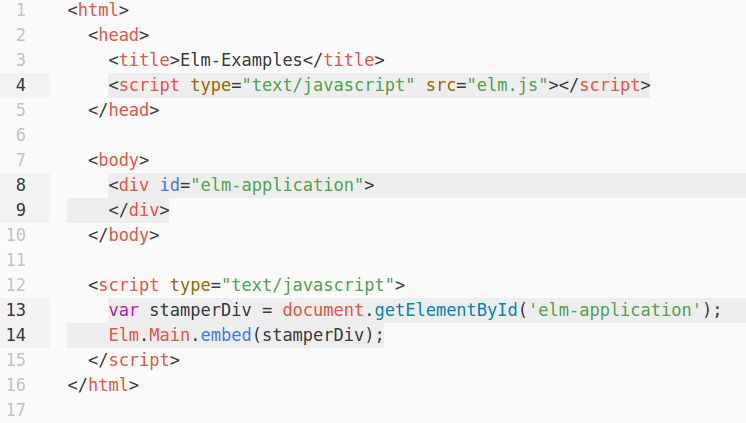
\includegraphics[scale=0.4]{img/elm-make_include_in_index.png}
%\caption{Grundgerüst eines\ac{HTML}-Dokumentes, um die Elm Applikation zu laden}\label{fig:html-boilerplate}
%\end{figure}
%
%\begin{figure}[htb]
%\centering
%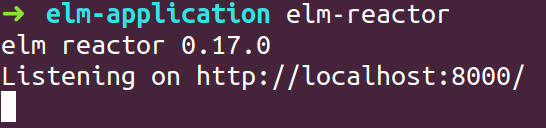
\includegraphics[scale=0.4]{img/elm-reactor.png}
%\caption{Der gestartete Elm-Webserver}\label{fig:elm-reactor}
%\end{figure}
%
%\noindent\textbf{Manueller Grundaufbau}\\
%Überlässt man dem Compiler das Einbinden der erzeugten \ac{JS}-Datei, so ist die gesamte Elm-Applikation im Vordergrund. Das ist nicht immer wünschenswert oder gar praktikabel. Einerseits, da externe Quellen für \ac{CSS} und \ac{JS} über natives Elm nicht reibungslos geladen werden können, andererseits weil nicht immer der gesamte darzustellende \ac{HTML}-Code nur in Elm geschrieben wurde. Dementsprechend gibt es auch die Möglichkeit, eine \ac{HTML}-Datei als Gerüst zu erzeugen, in die gezielt der \ac{JS}-Code der Elm-Applikation injiziert wird. Das Gerüst ist vollständig wie eine klassische \ac{HTML}-Datei aufgebaut. Abbildung~\ref{fig:html-boilerplate} zeigt das Grundgerüst des \ac{HTML}-Dokumentes. Codezeile $4$ bindet die kompilierte Elm-Datei. Der \ac{DOM}-Knoten in welchen die Applikation injiziert wird, ist in Zeile $8$ definiert. Das injizieren der Applikation geschieht in den Zeilen $13$ bis $14$ und erhält als Parameter den zuvor erwähnten \ac{DOM}-Knoten. Um die Elm-Applikation einfügen zu können, muss die Elm-Datei vorher in der Kommandozeile kompiliert werden mit dem Kommando $elm-make\,Datei.elm\,--output=elm.js$.
%Bei dieser Art der Initialisierung kann nun noch zwischen drei weiteren Darstellungen unterschieden werden:
%
%\begin{enumerate}
%\item$fullscreen$: Der erzeugte Code der Applikation wird in den Body-Tag einer\ac{HTML}-Datei geladen und überschreibt den sonstigen\ac{HTML}-Code.
%
%\item$embed$: Der erzeugte Code der Applikation wird in den übergebenen DOM-Knoten geladen.
%
%\item$worker$: Initialisiert die Applikation ohne grafische Benutzeroberfläche.
%\end{enumerate}
%Der Vorteil bei Version 2, so wie es auch in der Abbildung~\ref{fig:html-boilerplate} realisiert wurde, ist, dass auch nur kleine Teile der gesamten Applikation in Elm implementiert werden können. Überlegt man ein bestehendes, möglicherweise komplexes Projekt zu portieren, genügt es kleinere Teile Stück für Stück zu portieren. Es muss nicht befürchtet werden, große Teile der bestehenden Applikation während der Portierung nutzlos zu machen. Ein weiterer Vorteil ist, dass externes\ac{CSS} und\ac{JS} in dem \ac{HTML}-Dokument über die \ac{HTML}-eigenen $<script>$-Tags geladen werden kann.
%Zusätzlich zum Grundgerüst der $elm.html$ muss nun noch das Grundgerüst der eigentlichen Elm-App erstellt werden. Wie im Kapitel \nameref{sec:grundlagen} beschrieben, ist Elm nach einem \ac{MVU}-Konzept aufgebaut. Entsprechend sind das die unbedingt notwendigen Funktionen, die es zu realisieren gilt. Das standardmäßig mitgelieferte Paket $elm-lang/html$ liefert die sogenannten $Html.App$-Funktionen. Diese kümmern sich um die Bereitstellung und Auslieferung der Applikation, so dass sich Entwickler ganz auf die eigentliche Programmierung konzentrieren können. Dabei variieren stets die Übergabeparameter, wodurch die Applikation leicht erweitert und komplexer werden kann, ohne Neulinge direkt abzuschrecken. So verlangt die Funktion $Html.App.beginnerProgram$ nur die bekannten Funktionen $model$, $view$ und $update$. Hierbei können jedoch keine asynchronen Funktionen wie \ac{HTTP}-Requests genutzt werden.
%Dafür gibt es die erweiterte Funktion $Html.App.program$, die als vierten Übergabeparameter sogenannte $subscriptions$ erwartet. $Subscriptions$ werden für die Kommunikation zwischen Elm und \ac{JS}, sowie Verbindungen über Websockets genutzt.
%Die dritte und letzte Möglichkeit ist die Funktion $Html.App.programWithFlags$. Hierbei wird die Übergabe eines initialen $Models$ an die Elm-Applikation ermöglicht, um den Zustand der Applikation dynamisch setzen zu können.
%\begin{figure}[ht]
%\centering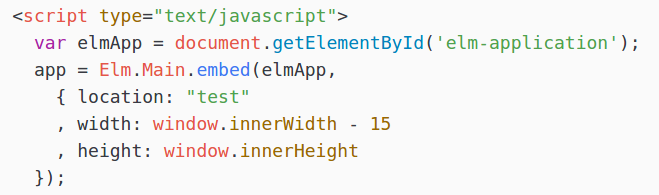
\includegraphics[scale=0.6]{img/programWithFlags_pass_data.png}
%\caption{Eine beispielhafte Initialisierung der Elm-Applikation mit übergebenen Werten}\label{fig:programWithFlags2}
%\end{figure}
%Abbildung~\ref{fig:programWithFlags2} zeigt das Grundgerüst einer Elm-Applikation mit der Implementierung der Funktion $Html.App.programWithFlags$. Die $main$ Funktion erstellt dabei die eigentliche Applikation, während die Funktionen $model$, $view$ und $update$ jeweils den Zustand und die gewünschte Darstellung der Applikation beschreiben, sowie vorgeben, wie mit der Interaktion durch den Benutzer umgegangen wird. Die Funktion $subscription$ gibt in diesem Stand noch keinerlei Daten weiter und stellt eine Dummy-Funktion dar. $initialModel$ erzeugt beim Aufruf ein Model mit initialen Werten, die dem Modeltypen ($type\,alias\,Model$) entsprechen müssen. Durch das Grundgerüst der $elm.html$ und $Main.elm$-Datei kann die Applikation nun schrittweise erweitert und Funktionen hinzugefügt werden. Zuletzt wird der erzeugte Code modularisiert.


%\subsubsection{Konstruktion und Überführung des Views}
%\label{sec:Konstruktion des Views}
%Damit \ac{HTML}-Elemente erzeugt werden können, werden die gleichnamigen Funktionen aus der Bibliothek $elm-lang/html$ genutzt. Im Zuge dessen wird die Bibliothek installiert und in die $*.elm$-Datei importiert. Mit Hilfe des Keywords $exposing$ wird eine Liste der Funktionen erzeugt, die in den aktuellen Namensraum der Applikation geladen werden sollen. Diese Liste wird mit den verwendeten Funktionsnamen zur Erstellung der \ac{HTML}-Elemente gefüllt, so dass die \ac{HTML}-Elemente ohne die Definition des ursprünglichen Namensraum $Html$ genutzt werden können.
%\begin{figure}[htb]
%\centering
%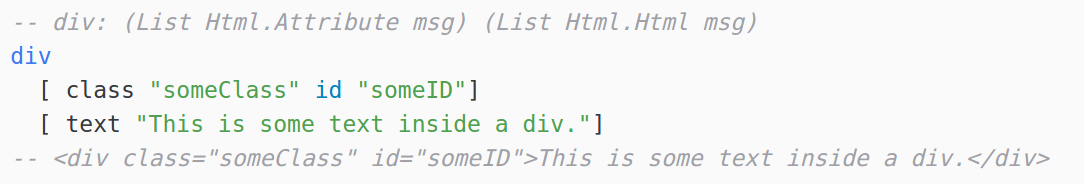
\includegraphics[scale=0.3]{img/div_elm_to_html.png}
%\caption{Resultat des Elm-Codes in \ac{HTML}}\label{fig:elm-to-html}
%\end{figure}

%Wie bereits erwähnt, hat erzeugt jede Funktion das gleichnamige \ac{HTML}-Element als äquivalent. Ein $div$-Element wird dementsprechend mit dem Aufruf der Funktion $div\,[\,][\,]$  erzeugt. Es ist erkannbar, dass die Funktion zwei Listen als Übergabeparameter erwartet. Die erste Liste enthält dabei optional sämtliche Attribute, die das \ac{HTML}-Element besitzen soll. Dazu gehören beispielsweise $class$ oder $href$. Die zweite Liste kann optional weitere \ac{HTML}-Elemente enthalten, um geschachtelte Konstrukte zu erzeugen. Die Signatur für die $div$-Funktion kann in Abbildung~\ref{fig:elm-to-html} betrachtet werden. Die Abbildung zeigt ferner, die Repräsentation von Elm-Code gegenüber dem daraus resultierenden \ac{HTML}-Code. Auch ist beispielhaft die Zuweisung einer Klasse ($class$) zu sehen. Auffällig sind die fehlenden $Tag$s des \ac{HTML}-Codes. Diese werden offenbar erst während der Kompilierung erzeugt. In Elm ist lediglich das Einrücken und schachteln der Funktionen von Bedeutung, um das entsprechende \ac{HTML}-Konstrukt zu erzeugen.
%\begin{figure}[htb]
%\centering
%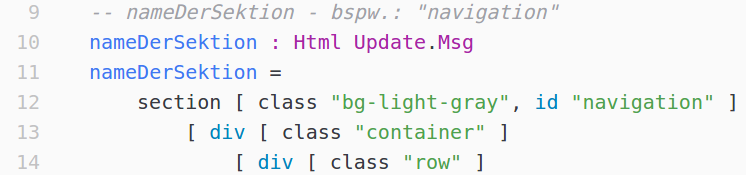
\includegraphics[scale=0.3]{img/elm-html-sections.png}
%\caption{Deklaration einer Sektion des Views in Elm}\label{fig:elm-view-section}
%\end{figure}

%Mit Hilfe des Tools $html-to-elm$ kann fertiger \ac{HTML}-Code automatisch in Elm-Code überführt werden. Das Tool wird für jede Sektion angewandt, um Zeit zu sparen und gleichzeitig die Funktionalität des Tools zu überprüfen. Für jede Sektion wird eine gleichnamige Funktion angelegt, die dem Muster in Abbildung~\ref{fig:elm-view-section} folgt. Die $id$ eines \ac{HTML}-Elementes könnte entsprechend stets für den Funktionsnamen $nameDerSektion$ genutzt werden, da dieses Attribut ohnehin einzigartig in einem gesamten \ac{HTML}-Dokument vorkommt und eine klare Namensgebung liefert.


%Das erste sichtbare Modul der fertigen SPA ist die Navigationsleiste. Sie soll dem Nutzer die Möglichkeit bieten schnell und einfach einen Überblick über die vorhandenen Themen auf der Webseite zu erhalten und direkt mit einem Klick auf den Reiter zu einem Thema zu springen. Damit die Navigation während des gesamten Besuches möglich ist, soll die Navigationsleiste `fixed` sein, also am oberen Bildschirmrand fest verankert bleiben und mit scrollen.
%Jedes Modul der dargestellten Seite besteht aus\ac{HTML}-Code. Folglich müssen\ac{HTML}-Tags mit Elm generiert werden. Seit dem neuesten Release von Elm (Version 0.17) wurden einige Pakete die sich für die Webentwicklung nutzen lassen zusammengeführt in das Paket `elm-lang/html`. Es erlaubt die Erzeugung von\ac{HTML} und\ac{CSS} mit nativem Elm-Code. In Elm können\ac{HTML}-Tags mit bereitgestellten Funktionen aus diesem Paket erzeugt werden. Ein\ac{HTML} `div`-Tag wird mit der gleichnamigen Funktion `div` erzeugt. Die Funktion erwartet zusätzlich zwei Argumente. Einerseits eine Liste von\ac{HTML}-Attributen wie `class`, `id` oder `href`, andererseits eine Liste von weiteren\ac{HTML}-Tags, insofern Code geschachtelt wird. Die Signatur für diese Funktion lautet wie folgt:
%`div (List Html.Attribute msg) (List Html.Html msg)`
%Entsprechend dieser Signatur wird in Abbildung XY gezeigt, wie die `div`-Funktion in Elm nach der Kompilierung in\ac{HTML} dargestellt wird.
%Nicht nur die Erstellung eines\ac{HTML}-Tags, sondern auch die Zuweisung von Attributen ist in Elm eine Funktion. So sieht man in Abbildung XY ebenso, wie eine Klasse (`class`) und ID einem Element hinzugefügt wird. Da in Elm sämtliche Funktionen „pure functions“, also reine Funktionen sind, hat der Entwickler die Sicherheit, dass das Resultat der Funktion immer gleich bleibt.
%Des Weiteren ist es möglich die\ac{HTML}-Elemente nativ in Elm mit\ac{CSS}-Styling zu versehen. Dafür wird die gleichnamige Funktion `style` aus dem Paket genutzt. Auch diese Funktion erwartet eine Liste von Argumenten, jeweils mit einem Schlüssel (hier:\ac{CSS}-Eigenschaft) und dem dazugehörigen Wert. Zur Zeit ist es nicht problemlos möchlich nativ in Elm eine externe\ac{CSS}-Datei zu integrieren. Corey Trampe (https://gist.github.com/coreytrampe/a120fac4959db7852c0f) hat eine Möglichkeit gefunden, jedoch wird bei dieser Lösung die Seite zunächst ohne jegliches Styling dargestellt, während ein asynchroner Request die externe\ac{CSS}-Datei lädt. Sobald dieser Vorgang abgeschlossen ist, wird das heruntergeladene Styling angewandt. Der zeitliche Abstand zwischen initialem Laden und der Anwendung des Styles hat ein sichtbares „flackern“ zur Folge, wodurch eine Nutzung in einem fertigen System entfällt. Alternativ werden alle zu ladenden\ac{CSS}-Dateien im\ac{HTML}-Grundgerüst über den\ac{HTML}-Tag `link` eingebunden.


%\subsubsection{Überführung des Views}
%\label{sec:Überführung des Views}
%Für die Darstellung einer SPA wird ein fertiges und kostenloses Theme von `startbootstrap.com` verwendet. Im Zuge dessen werden alle verfügbaren Dateien heruntergeladen und die zuvor erstellten Dateien `elm.html` und `Main.elm` in denselben Ordner verschoben.
%Das Grundgerüst der `elm.html` muss nun in die `index.html` überführt werden, so dass die Elm-Applikation weiterhin in den vorhandenen \ac{HTML}-Code injiziert wird.
%Zunächst einmal muss der \ac{HTML}-Code des Themes in ausführbaren Elm-Code umgeschrieben werden, damit Elm Zugriff auf den kompletten `view` bekommt. Nur so kann Elm die Interaktion des Benutzers mit den\ac{HTML}-Elementen abfangen und entsprechend darauf reagieren. Um nicht den kompletten\ac{HTML}-Code der `index.html` per Hand in Elm-Code überführen zu müssen, wird das Tool `html-to-elm` genutzt (http://mbylstra.github.io/html-to-elm/). Dieses Online-Tool erlaubt es\ac{HTML}5-konformen Code in lauffähigen Elm-Code zu überführen. Der erzeugte Elm-Code wird dann in der `Main.elm`-Datei von der `view`-Funktion zurückgegeben., muss also entsprechend dort eingefügt werden.
%Um Modularität zu gewährleisten, wird jede Sektion der SPA, wie zum Beispiel die Navigation, die Team-Sektion oder der Footer im ersten Schritt in eine eigene Funktion ausgelagert. Jede dieser Funktionen wird dann in der `view`-Funktion aufgerufen und ergibt am Ende die gesamte Webseite. Auf diese Weise können die einzelnen Teile der SPA unabhängig voneinander modifiziert und auf Korrektheit überprüft werden. Im nächsten Schritt wird der gesamte View-Code modularisiert.



%\subsubsection{Modularisierung}
%\label{sec:Modularisierung}
%Damit ein Entwickler den Überblick über den vorhandenen Quellcode behält ist es sinnvoll einzelne Teile der Applikation in mehrere Dateien und Ordner zu verschieben. Eine solche Strukturierung hilft dabei die womöglich fehlerbehafteten Teile der Applikation zu finden und beispielsweise die Programmlogik noch deutlicher von der Applikationsdarstellung zu trennen. Dabei werden die einzelnen Funktionen des Views, also die für die Darstellung verantwortlichen Programmteile, ausgelagert in eigene Module. Dasselbe wird für die `Update` und `Model` relevanten Funktionen durchgeführt. Die notwendigen Funktionen eines jeden Moduls werden dann im Gegenzug vom Hauptmodul importiert und an den entsprechenden Stellen aufgerufen.\\\\
%\noindent\textbf{View}\\
%Jede bisherige Funktion aus dem View wird in den Ordner `View` verschoben und als gleichnamiges Modul benannt. Jedes Modul bekommt dabei den Namen des Ordners in dem es zu finden ist, gefolgt vom Namen des Views, dass es darstellt. Das für die Navigation verantwortliche Modul wird  entsprechend mit `module View.Navigation exposing (view)` initialisiert und gibt die Funktion `view` an jedes importierende Modul frei.
%Dieser Schritt dient lediglich der besseren Strukturierung des Quellcodes und der Vereinfachung für den Entwickler. Abbildung XY zeigt die Haupt-`view`-Funktion nachdem sämtliche Teile des `View`s modularisiert und entsprechend importiert wurden.\\\\
%\noindent\textbf{Update}\\
%Auch die Programmlogik kann modularisiert werden und wird dafür in den Unterordner $Update$ verschoben. Hierfür werden sämtliche Typdeklarationen ($Msg$), sowie die dazugehörige Funktion $update$ in das neue Modul `Update.Update` verschoben und auch die notwendigen Pakete hinzugefügt. Von außen kann auf das $Update$-Modul, nachdem es importiert wurde, mit dem Namespace $Update$ zugegriffen werden.\\\\
%\textbf{Model}\\
%Letztlich wird noch das $model$, das sämtliche Daten die den Status der Applikation beschreiben enthält, in ein eigenes Modul im Unterordner $Model$ überführt. Die Einbindung dieses Moduls funktioniert analog zur Modularisierung von $Update$ und $View$.
%Mit Hilfe dieser Modularisierung wird das angestrebte \ac{MVU}-Konzept von Elm besonders deutlich.

%\subsubsection{Asynchrones Laden}
%\label{sec:Asynchrones Laden - Analyse}
%Klickt man innerhalb der Portfolio-Sektion der Webseite auf ein Element, öffnet sich ein Modal in dem weitere Informationen dargestellt werden. Die bestehende Elm-Applikation wird nun um das Feature des asynchronen Ladens von Informationen erweitert, die anschließend in dem geöffneten Modal angezeigt werden.
%Zunächst muss das $model$ erweitert und angepasst werden, da dies die einzige Möglichkeit in einer Elm-Applikation ist, Daten beziehungweise den Status der Applikation zu speichern. Das `model` bekommt entsprechend ein weiteres Feld $async\_content$ vom Typ $String$.
%Bei einem Klick auf eines der Portfoliobeiträge soll entsprechend das Modal geöffnet und ein Titel präsentiert werden. In diesem Beispiel wird über eine externe API ein zufälliger String angefordert, vom Server generiert und dann an die Elm-Applikation zurückgegeben. Ebenso wäre es möglich einen Server für das Backend zu erstellen, auf dem eine Datenbank läuft, so dass Daten asynchron angefordert werden können. In diesem Fall ist es jedoch nicht notwendig ein zusätzliches Backend zu konfigurieren.
%Ein solcher asynchroner Request stellt im Grunde eine Verletzung des Konzeptes von Elm dar, dass es keinerlei Seiteneffekte gibt. Da nicht bekannt ist, wann der Request endet und welchen Status die Antwort besitzt (Failed, Success, ..?), ist zunächst nicht vorhersehbar, wie der Status der Applikation nach dem Request aussehen wird. Um dieses Problem zu vermeiden, ist es notwendig alle möglichen Fälle , also den Fall einer erfolgreichen, sowie fehlerhaften Übertragung, zu behandeln. Auf diese Weise ist gewährleistet, dass die Applikation sich nicht plötzlich in einem nicht definierten Zustand befindet.
%Einen asynchronen Request in Elm auszuführen bedarf mindestens zweier zusätzlicher Funktionen und der Importierung der Bibliotheken $Http$, $Json.Decode$ und $Task$. Des Weiteren muss der Klick auf das Portfolio-Element abgefangen werden. Dafür gibt es die $onClick$ Funktion aus der $Html.Events$-Bibliothek. Sie bekommt die auszuführende Funktion als Parameter, sieht also wie folgt aus: `onClick Update.GetRandomString`. Die möglichen `Types` von eingehenden Nachrichten (`Msg`/Klicks) wird erweitert um `GetRandomString`, sowie auch die `update`-Funktion um diesen Typ erweitert werden muss. Der entsprechende `update`-Fall `GetRandomString` gibt dann das `model`, sowie einen Effekt `fetchAsync` zurück. Die Definition dieses Effektes ist der Grund, weshalb hier von einem `managed Effect` die Rede ist und der Seiteneffekt kontrolliert verläuft. `fetchAsync` ist hierbei erneut eine Funktion, die eine Nachricht (`Msg`) an die `update`-Funktion mit dem Ergebnis des Requests zurückgibt . Elm führt den Request in Form eines `Task` aus und erwartet eine Funktion für den Fall einer erfolgreichen Übertragung, sowie eine Funktion für jeglichen Fehlerfall. In beiden Fällen wird die entsprechende Funktion ausgeführt und an die `update`-Funktion zurückgegeben. Hier wird, insofern notwendig, ein neues `model` mit veränderten Werten erzeugt und letztlich das Ergebnis auf dem Bildschirm des Nutzers sichtbar gemacht.\\



\subsection{Auswertung}
\label{sec:Auswertung}
- Das bedeutet, dass nativer Code in Elm kürzer und weniger anfällig für Flüchtigkeitsfehler wie beispielsweise das Schließen eines Tags ist. Der Entwickler wird weniger syntaktische Fehler machen.\\


\begin{table}[h]
\centering
\begin{tabular}{ | l | c | }
	\hline
	\textbf{Kriterium} & \textbf{Erfüllt}\\
	\hline
	1. Entwicklungsgeschwindigkeit & \\
	1.1 & \checkmark\\
	\hline
	2. Wartbarkeit & \\
	2.1  & \checkmark\\
	\hline
	3. Zuverlässigkeit & \\
	3.1  & \checkmark\\
	3.2  & \checkmark\\
	3.3  & \checkmark\\
	\hline
	4. Portabilität & \\
	4.1  & ausstehend\\
	\hline
	5. Effizienz & \\
	5.1  & \checkmark\\
	5.2  & ausstehend\\
	\hline
	6. Wiederverwendbarkeit & \\
	6.1  & \checkmark\\
	\hline
	7. Modularität & \\
	7.1  & \checkmark\\
	7.2  & \checkmark\\
	\hline
	8. Lesbarkeit & \\
	8.1  & \checkmark\\	
	\hline
	9. Dateigröße & \\
	9.1  & ausstehend\\
	\hline
	10. Interoperabilität & \\
	10.1  & \checkmark\\
	10.2  & Nein/Nur bedingt\\
	\hline
	11. Asynchrones Laden & \\
	11.1  & \checkmark\\
	\hline
\end{tabular}
\caption{Auswertung der Versuchskriterien}
\label{tab:Auswertungstabelle}
\end{table}
%TODO: Importieren der schriftlichen Auswertung der Tabelle~\ref{tab:Auswertungstabelle}

 1.1. Elm hat leicht erlernbare Grundkonzepte, die adaptiert und erweiterbar sind, um Produktivität für die Entwickler zu gewährleisten.
 
 2.1. Elm Code kann mindestens kommentiert werden, wenn nicht sogar eine Funktion zur automatischen Generierung von Signaturen einer Funktion existiert
 --> Kommentare können mit `--` (single-line) oder `{- a comment - }` erstellt werden. Eine vollautomatische, explizite Erstellung der Signaturen besteht derzeit nicht. Der Compiler wird jedoch nach dem Kompiliervorgang einen Signaturvorschlag geben. Dieser Vorschlag ist auf einer niedrigeren Ebene, als es eine Deklaration wäre, ist jedoch ausreichend und wesentlich sinnvoller als eine Signatur komplett unberücksichtigt zu lassen. Beispiel: Abbildung XY ($compiler_sig_suggestion$ + $compiler_own_sig$)
 ```
 type alias Model = { counter: Int }
 increaseModel: Model -> Model
 increaseModel model =
     {model | counter = model.counter + 1}
 
 vs. Kompiliervorschlag
 type alias Model = { counter: Int }
 increaseModel: { a | counter : number } -> { a | counter : number }
 increaseModel model =
     {model | counter = model.counter + 1}
 ```
 
 3.1. Die Erweiterungen des Editors oder der Compiler warnt spätestens bei der Kompilierung, wenn nicht bereits während der Entwicklung vor syntaktischen Fehlern
 --> Syntaktische Fehler werden vom Compiler erkannt und ein Fehler angezeigt. Der Fehler wird unterstützt durch einen Hinweis auf die mögliche Fehlerquelle (Abbildung XY – $Compiler_syntax_error$). Die Fehlermeldung wird erst nach der Kompilierung eingeblendet.
 ```
 div [ id "elm-view" ]
         [ Navigation.view model
             Header.view
         , Services.view]
 ```
 
 3.2. Gibt es keine Fehlermeldungen, wird die Applikation ohne Laufzeitfehler funktionieren
 --> Aufgrund der Garantien, dass es keine Seiteneffekte gibt und alle Variablen unveränderlich sind, ist die Korrektheit syntaktische und semantische Korrektheit des Codes gewährleistet. Lediglich die logische Implementierung eines Algorithmus kann noch Fehler aufweisen, dies kann jedoch nicht von einem Compiler überprüft werden.
 3.3. Fehlermeldungen werden sehr spezifisch auf das eigentliche Problem hinweisen
 --> Wie in Abbildung iii.i zu sehen ist, gibt der Compiler nicht nur an, in welcher Zeile ein Fehler gefunden wurde, sondern liefert zusätzlich noch einen Hinweis, worin eine wahrscheinliche Fehlerquelle liegt. In diesem Beispiel weißt der Compiler auf das fehlende Komma als Fehlerquelle hin.
 
 4.1  1. Die SPA wird auf allen gängigen Browsern fehlerfrei dargestellt
 --> AUSSTEHEND
 
 5.1. Der Kompiliervorgang wird nur wenige Sekunden dauern, jedoch mehr Zeit in Anspruch nehmen, als die herkömmliche Entwicklung mit reinem\ac{HTML},\ac{CSS} und\ac{JS}
 --> Bei der herkömmlichen Entwicklung ist kein expliziter Kompiliervorgang notwendig, stattdessen übernimmt der Browser die Darstellung des übergebenen\ac{HTML},\ac{CSS} und\ac{JS} Quellcodes. Der Kompiliervorgang der Elm-Applikation dauert wie in Abbildung XY  zu sehen ist im Durchschnitt XY Sekunden. Es wurde 10x gemessen, der höchste und niedrigste Wert gestrichen und dann das arithmetische Mittel der verbleibenden 8 Messungen ermittelt.
 
 5.2  2. Die erzeugte Elm-Applikation ist deutlich schneller während der Laufzeit
 --> AUSSTEHEND (Abbildung - Performance - Evtl. neu?)
 
 6. 1. Codeteilen lassen sich problemlos auslagern und wiederverwenden
 --> Der komplette View wurde von einer großen Darstellung in mehrere Funktionen unterteilt und letztlich in ein eigenes Modul überführt. Analog dazu wurden auch das Model, sowie die Update-Funktion ausgelagert. Das einmalig definierte `Model` kann in sämtlichen Modulen wiederverwendet werden, auch die einzelnen Funktionen eines jeden Moduls finden erneut Verwendung, insofern gewünscht.
 
 7.1. Ausgelagerte Codeteile sind isoliert voneinander und als einzelnes Modul nutzbar
 --> Diese Eigenschaft ist gegeben.
 7.2. Module können Funktionen nach außen verbergen
 --> Jedes Modul kann mit dem Stichwort `expose` einzelne Funktionen nach außen hin zugänglich machen. Das importierende Modul wiederum kann einzelne Funktionen in den derzeitigen globalen `Scope` laden.
 
 8.1. Die automatische Formatierung des Elm-Codes macht diesen lesbarer und spart Zeit
 --> Fehler werden Dank der Formatierung schnell sichtbar.
 
 9.1. Die Dateigröße der Elm-Applikation wird kleiner als bei vergleichbaren Frameworks ausfallen
 --> Die kompilierte Elm-Applikation hat eine Größe von etwa 300kb. Allerdings kann diese Größe um etwa 60Prozent verringert werden, wenn der Code `minified` wird.

10.1. Bestehende\ac{JS}-Skripte können mit der Elm-Applikation interagieren oder funktionieren bereits einwandfrei
--> Die Integration vorhandener\ac{JS}-Skripte verlief problemlos. Benötigt ein externes Skript Daten von der Elm-Applikation, so kann mit Hilfe von `Ports` eine gesicherte Kommunikation in beide Richtungen stattfinden.

10.2. Bestehender\ac{CSS}-Code kann nativ in Elm eingebunden werden
--> Das Einbinden von\ac{CSS} Quellen ist derzeit nicht ohne Probleme nativ in Elm möglich. Es verursacht ein „flackern“ und ist nicht für den Gebrauch in einem fertigen System geeignet.\ac{CSS}-Klassen und `inline-styling` sind jedoch nativ in Elm implementiert und erlauben ein Styling der Elemente. Externes\ac{CSS} muss jedoch über das Grundgerüst der\ac{HTML}-Datei eingebunden werden.

11.1. Elm erlaubt asynchrone Requests ohne Seiteneffekte zu erzeugen
--> Ein asynchroner Request stellt implizit einen Seiteneffekt dar, wird in Elm allerdings als gemanagter Seiteneffekt bezeichnet. In jedem Fall ist der Nutzer gezwungen eine Funktion bei einer fehlerhaften Übertragung zu übergeben, die dann die erwartenden Typen/Werte liefert.

\subsection{Fazit}
\label{sec:Fazit}

  
1. Installation sehr einfach
1. externe Abhängigkeiten werden automatisch installiert
2. Installation war schnell
3. Erklärung zur Installation war deutlich
2. Modularität möglich
1. Jedes View-Element als eigenes Modul
1. Paralleles arbeiten möglich
2. Entwickler bekommen nur die notwendigen Informationen für das Interface
3. Tools
1.\ac{HTML}2ELM sehr hilfreich
1. Kleinere Fehler
1. ' verursacht Fehler (Weiterfolgende Divs wurden vernachlässigt)
2. required --> required '' (wants Bool, got String); novalidate same
2. Elm-Compiler
1. Fehler von\ac{HTML}2ELM (2. Punkt) wurden sofort erkannt
2. Fehlende Funktionen für\ac{HTML} und\ac{CSS} Attribute wurden in den Fehlermeldungen vorgeschlagen („Did you mean Html.Attributes.required?“ für „required true“)
4. Erklärungen der Elm-Struktur in den Guides sehr gut